\section{服务模型}

\subsection{SOAP}

\subsubsection{SOAP的引入}
\begin{itemize}
    \item 现在我们有:
    \begin{itemize}
        \item 我们使用XML定义了Web Service中的消息交换格式
        \item 通过引入NameSpace使得XML中的元素(Element)/属性(Attribute)全球唯一且全球共享
        \item 通过Schema定义了数据类型(同上)
    \end{itemize}
    \item 下一个问题是:使用Web Service作为服务的具体实现技术,服务的发布/查找、调用,都需要通过互联网传递XML消息
    \begin{itemize}
        \item 一个可能的方法是,直接将XML作为文本载荷通过特定网络协议(HTTP,SMTP,FTP等)加以传递
        \item 为什么选择SOAP:提供了一种标准的方法,使得运行在不同平台并使用不同的技术和编程语言的应用程序可以互相进行通信
    \end{itemize}   
\end{itemize}

\subsubsection{什么是SOAP}
SOAP提供了一种标准的方法,使得运行在不同平台并使用不同的技术和编程语言的应用程序可以互相进行 XML 通信。从本质上来说,SOAP并不是一个网络传输协议,它仅仅是一个信息传递的概念性框架,在实际使用时,需要绑定具体的网络传输协议和上层的应用逻辑来创建关联。
\begin{itemize}
    \item SOAP使用XML定义了可扩展的消息架构,该消息架构提供了能够基于多种底层协议,进行信息交换的信息架构。
    \item SOAP基本上是一种无状态的单向消息交换范例。应用程序可以通过将这种单向交换与底层协议提供的功能和/或应用程序特定信息相结合来创建更复杂的交互模式(例如,请求/响应、请求/多个响应等)。
    \item SOAP提供在可扩展的方式下传递应用程序特定信息的框架和接收SOAP消息时SOAP节点执行的所有必需操作的完整描述。
    \item SOAP并不关心它所携带的应用相关数据的语义(就像信封不关心在信封中装的是支票还是邮件)、SOAP消息路由、可靠数据传输、防火墙穿越等问题。
\end{itemize}

\subsubsection{SOAP的两种使用方式}
\begin{figure}[H]
	\setcounter{subfigure}{0}
	\centering
	\vspace{-2em}	
	\subfloat[没有中间转发节点]{
	\begin{minipage}[t]{0.3\linewidth}
	\centering
	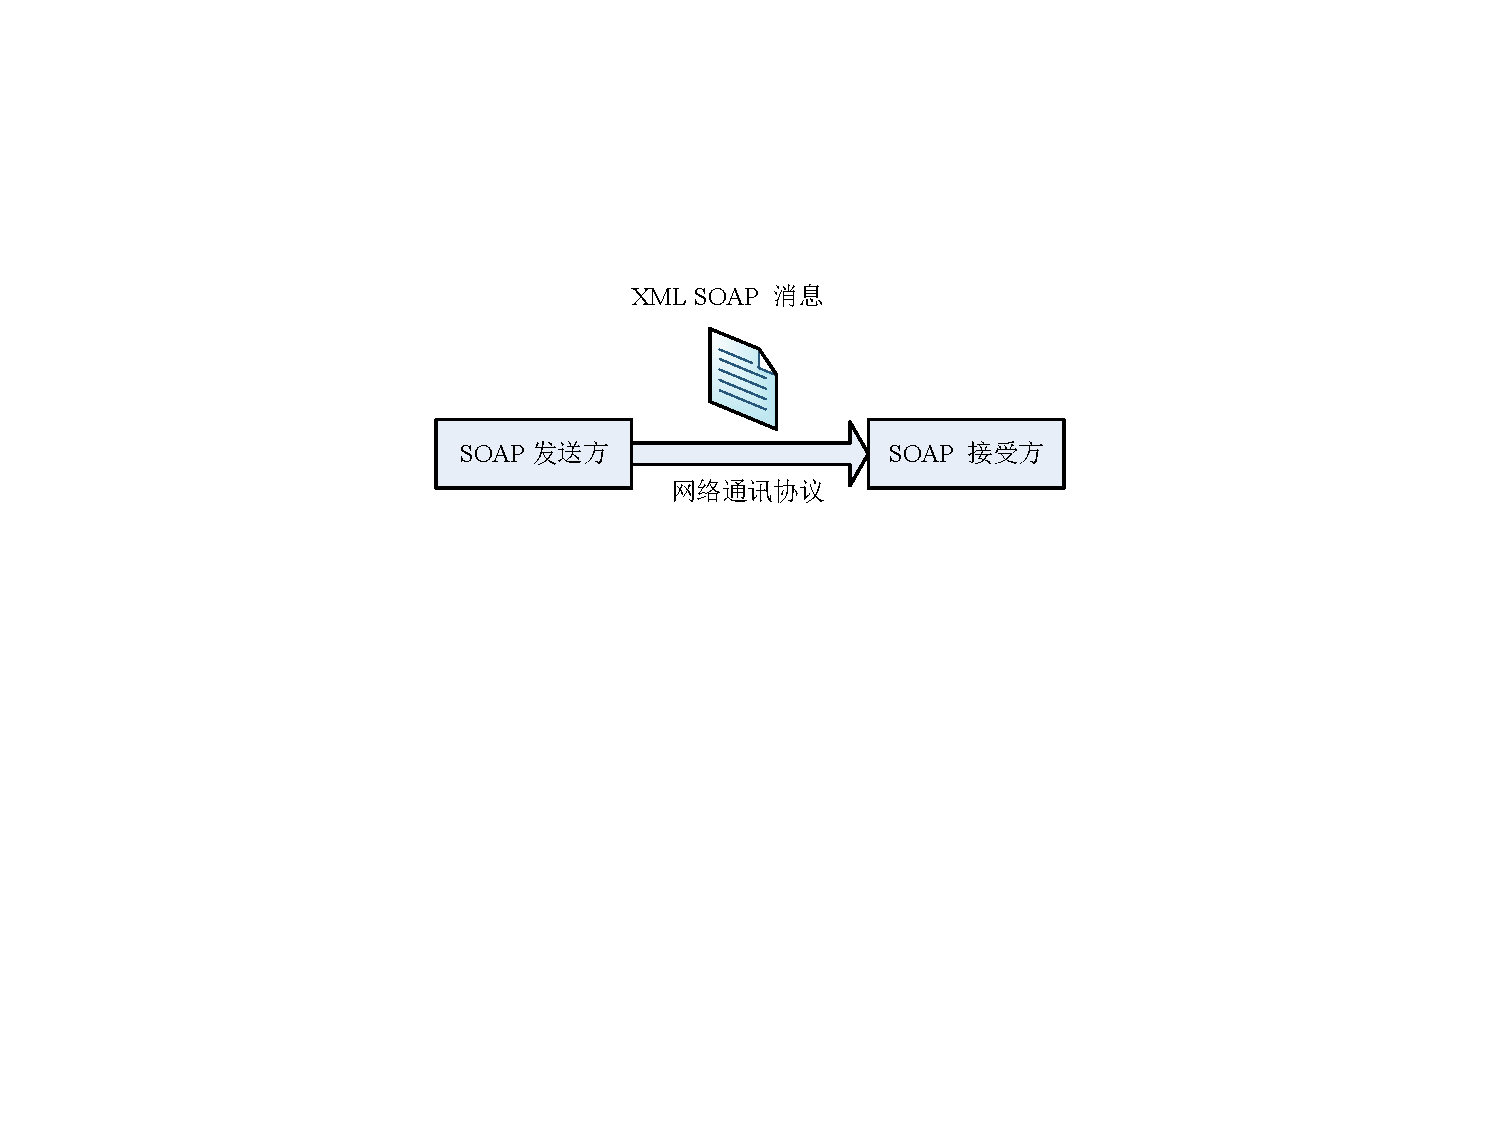
\includegraphics[width=0.97\linewidth]{images/SOAP没有中间转发节点.pdf}
	\end{minipage}
	}
    \subfloat[有多个中间转发节点]{
	\begin{minipage}[t]{0.66\linewidth}
	\centering
	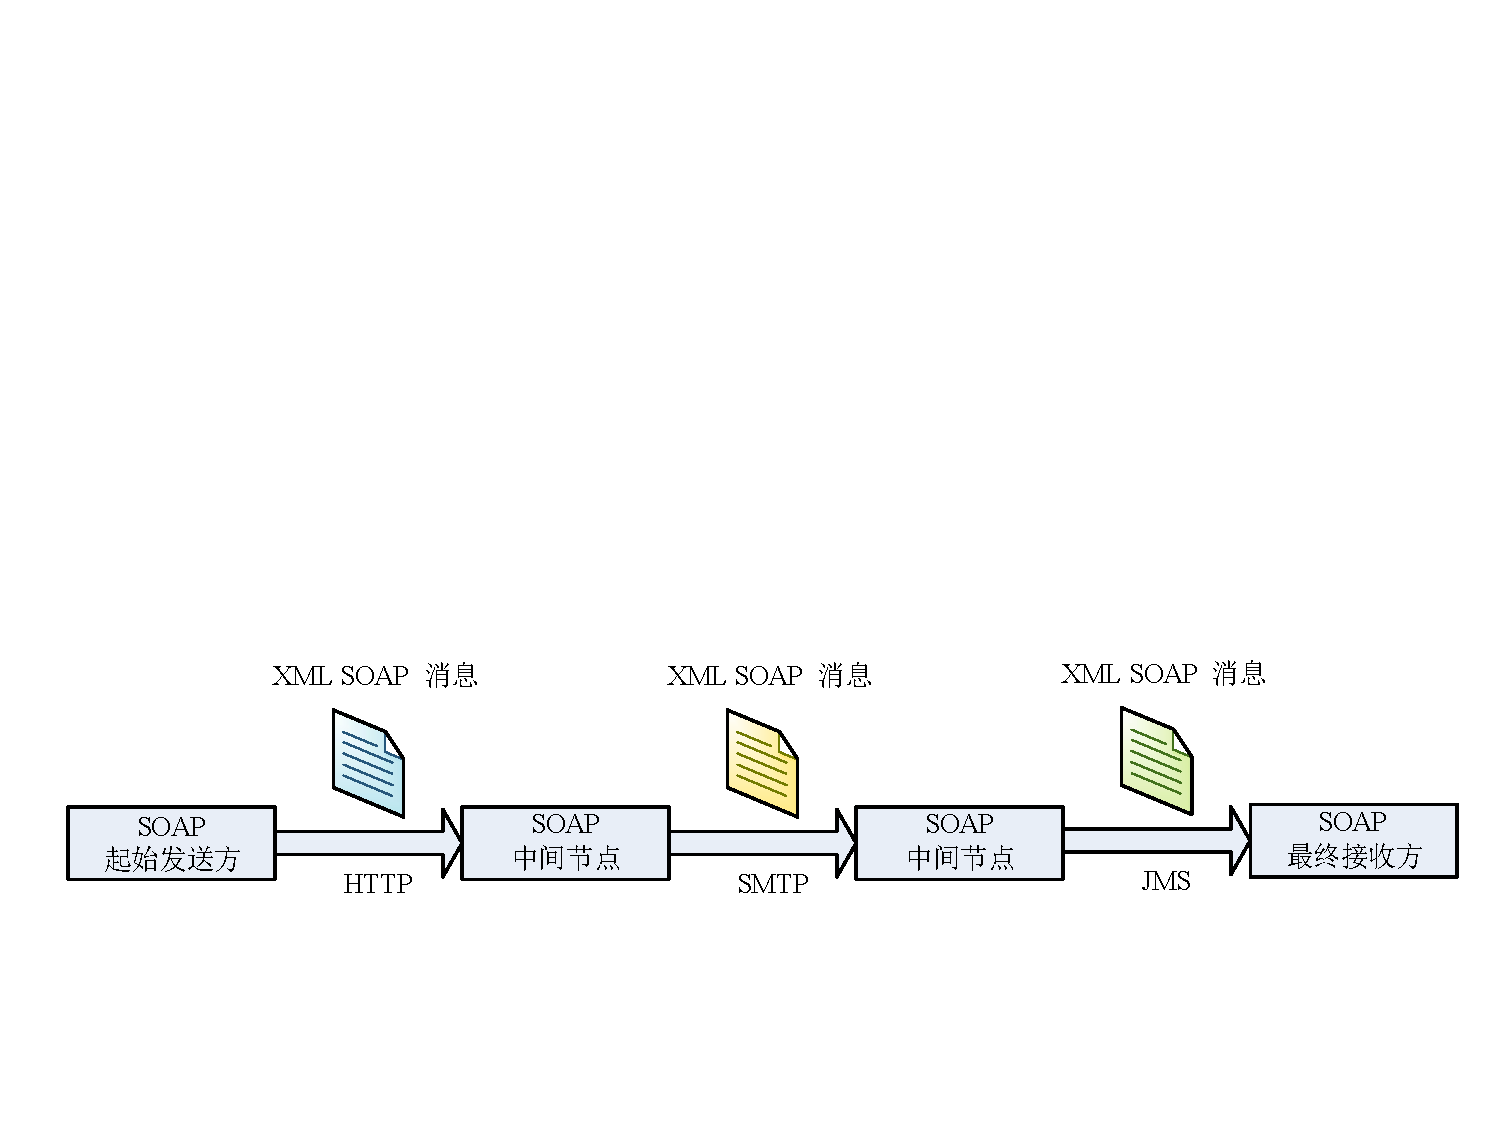
\includegraphics[width=0.93\linewidth]{images/SOAP有多个中间转发节点.pdf}
	\end{minipage}
	}
	\centering
	\vspace{-1.5em}
\end{figure}


\subsubsection{SOAP的两种交互模式}
RPC(远程过程调用)模式:
\vspace{-0.3em}
\begin{multicols}{2}
    \begin{itemize}
        \item 同步的请求/应答交互模式
        \item 发送请求并等待响应
    \end{itemize}
\end{multicols}
\vspace{-1em}

面向文档模式(大多数情况):
\begin{vwcol}[widths={0.3\textwidth,0.65\textwidth},rule=0pt]
    \hspace{1em}{\footnotesize$\bullet$}\hspace{0.5em}异步交互模式

    {\footnotesize$\bullet$}\hspace{0.5em}发送复杂的XML文档,并等待通知,结果会在处理后发回
\end{vwcol}


\subsubsection{SOAP结构}
\begin{figure}[H]
    \vspace{-0.5em}
	\centering
	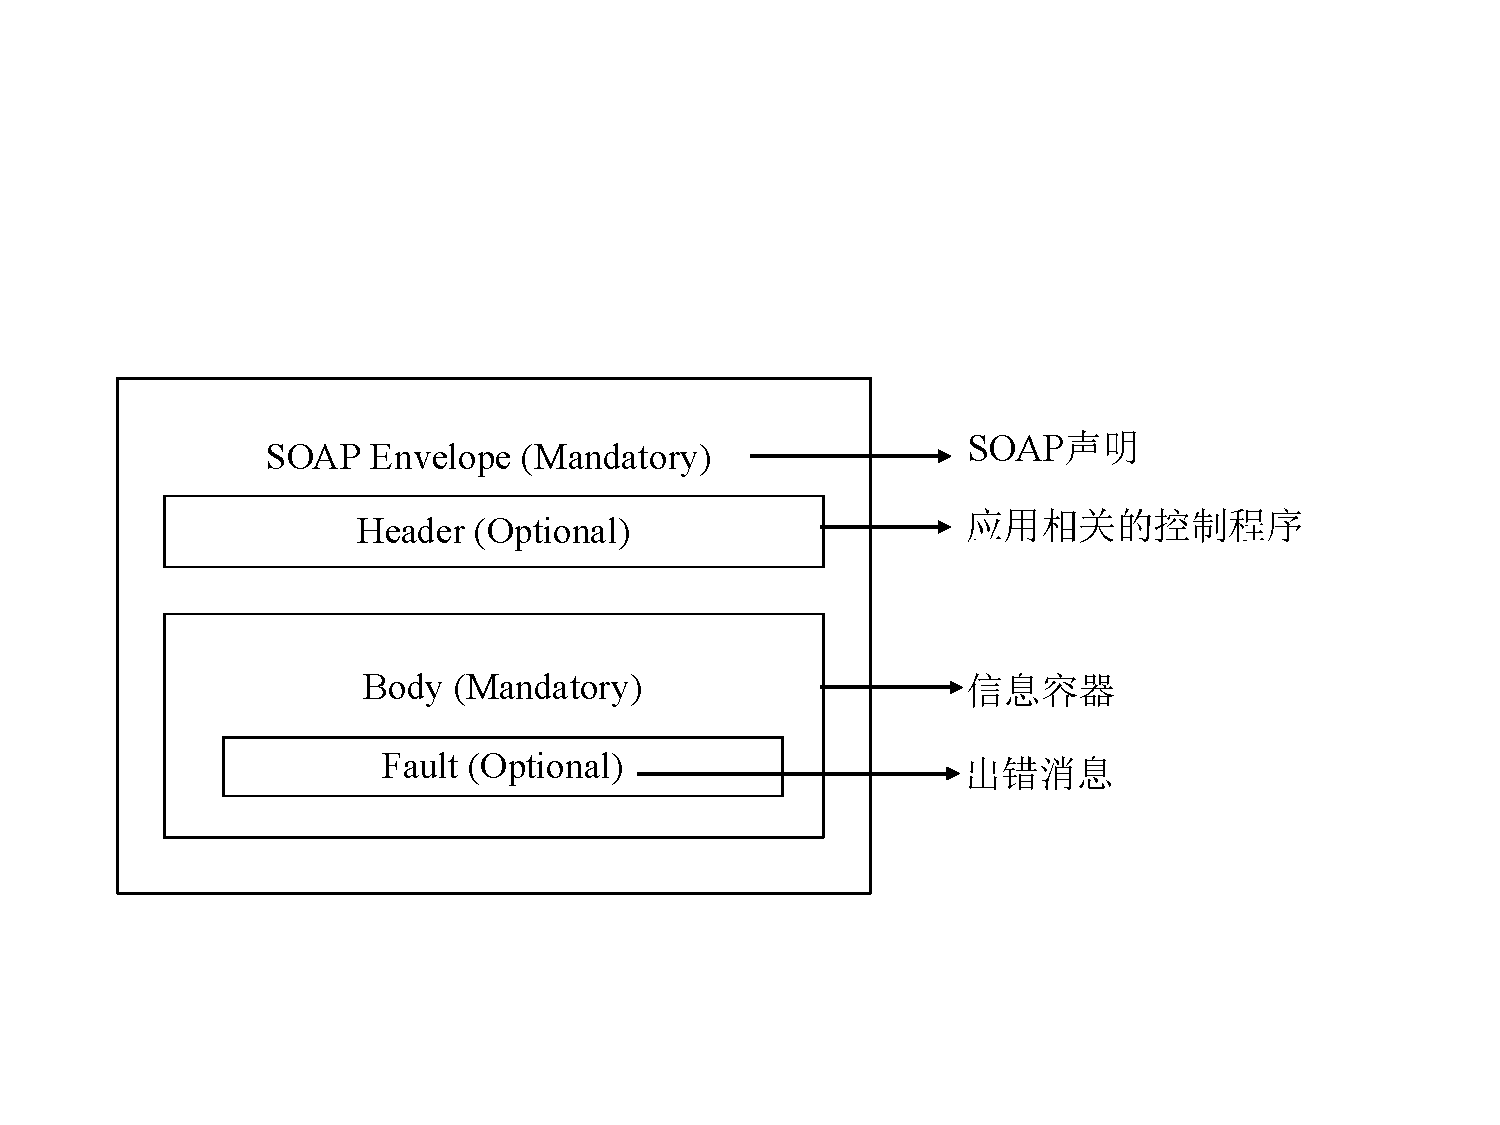
\includegraphics[width=0.7\textwidth]{images/SOAP结构.pdf}
    \vspace{-1em}
\end{figure}

\paragraph*{SOAP消息示例}~{} \par
\begin{figure}[H]
    \vspace{-0.5em}
	\centering
	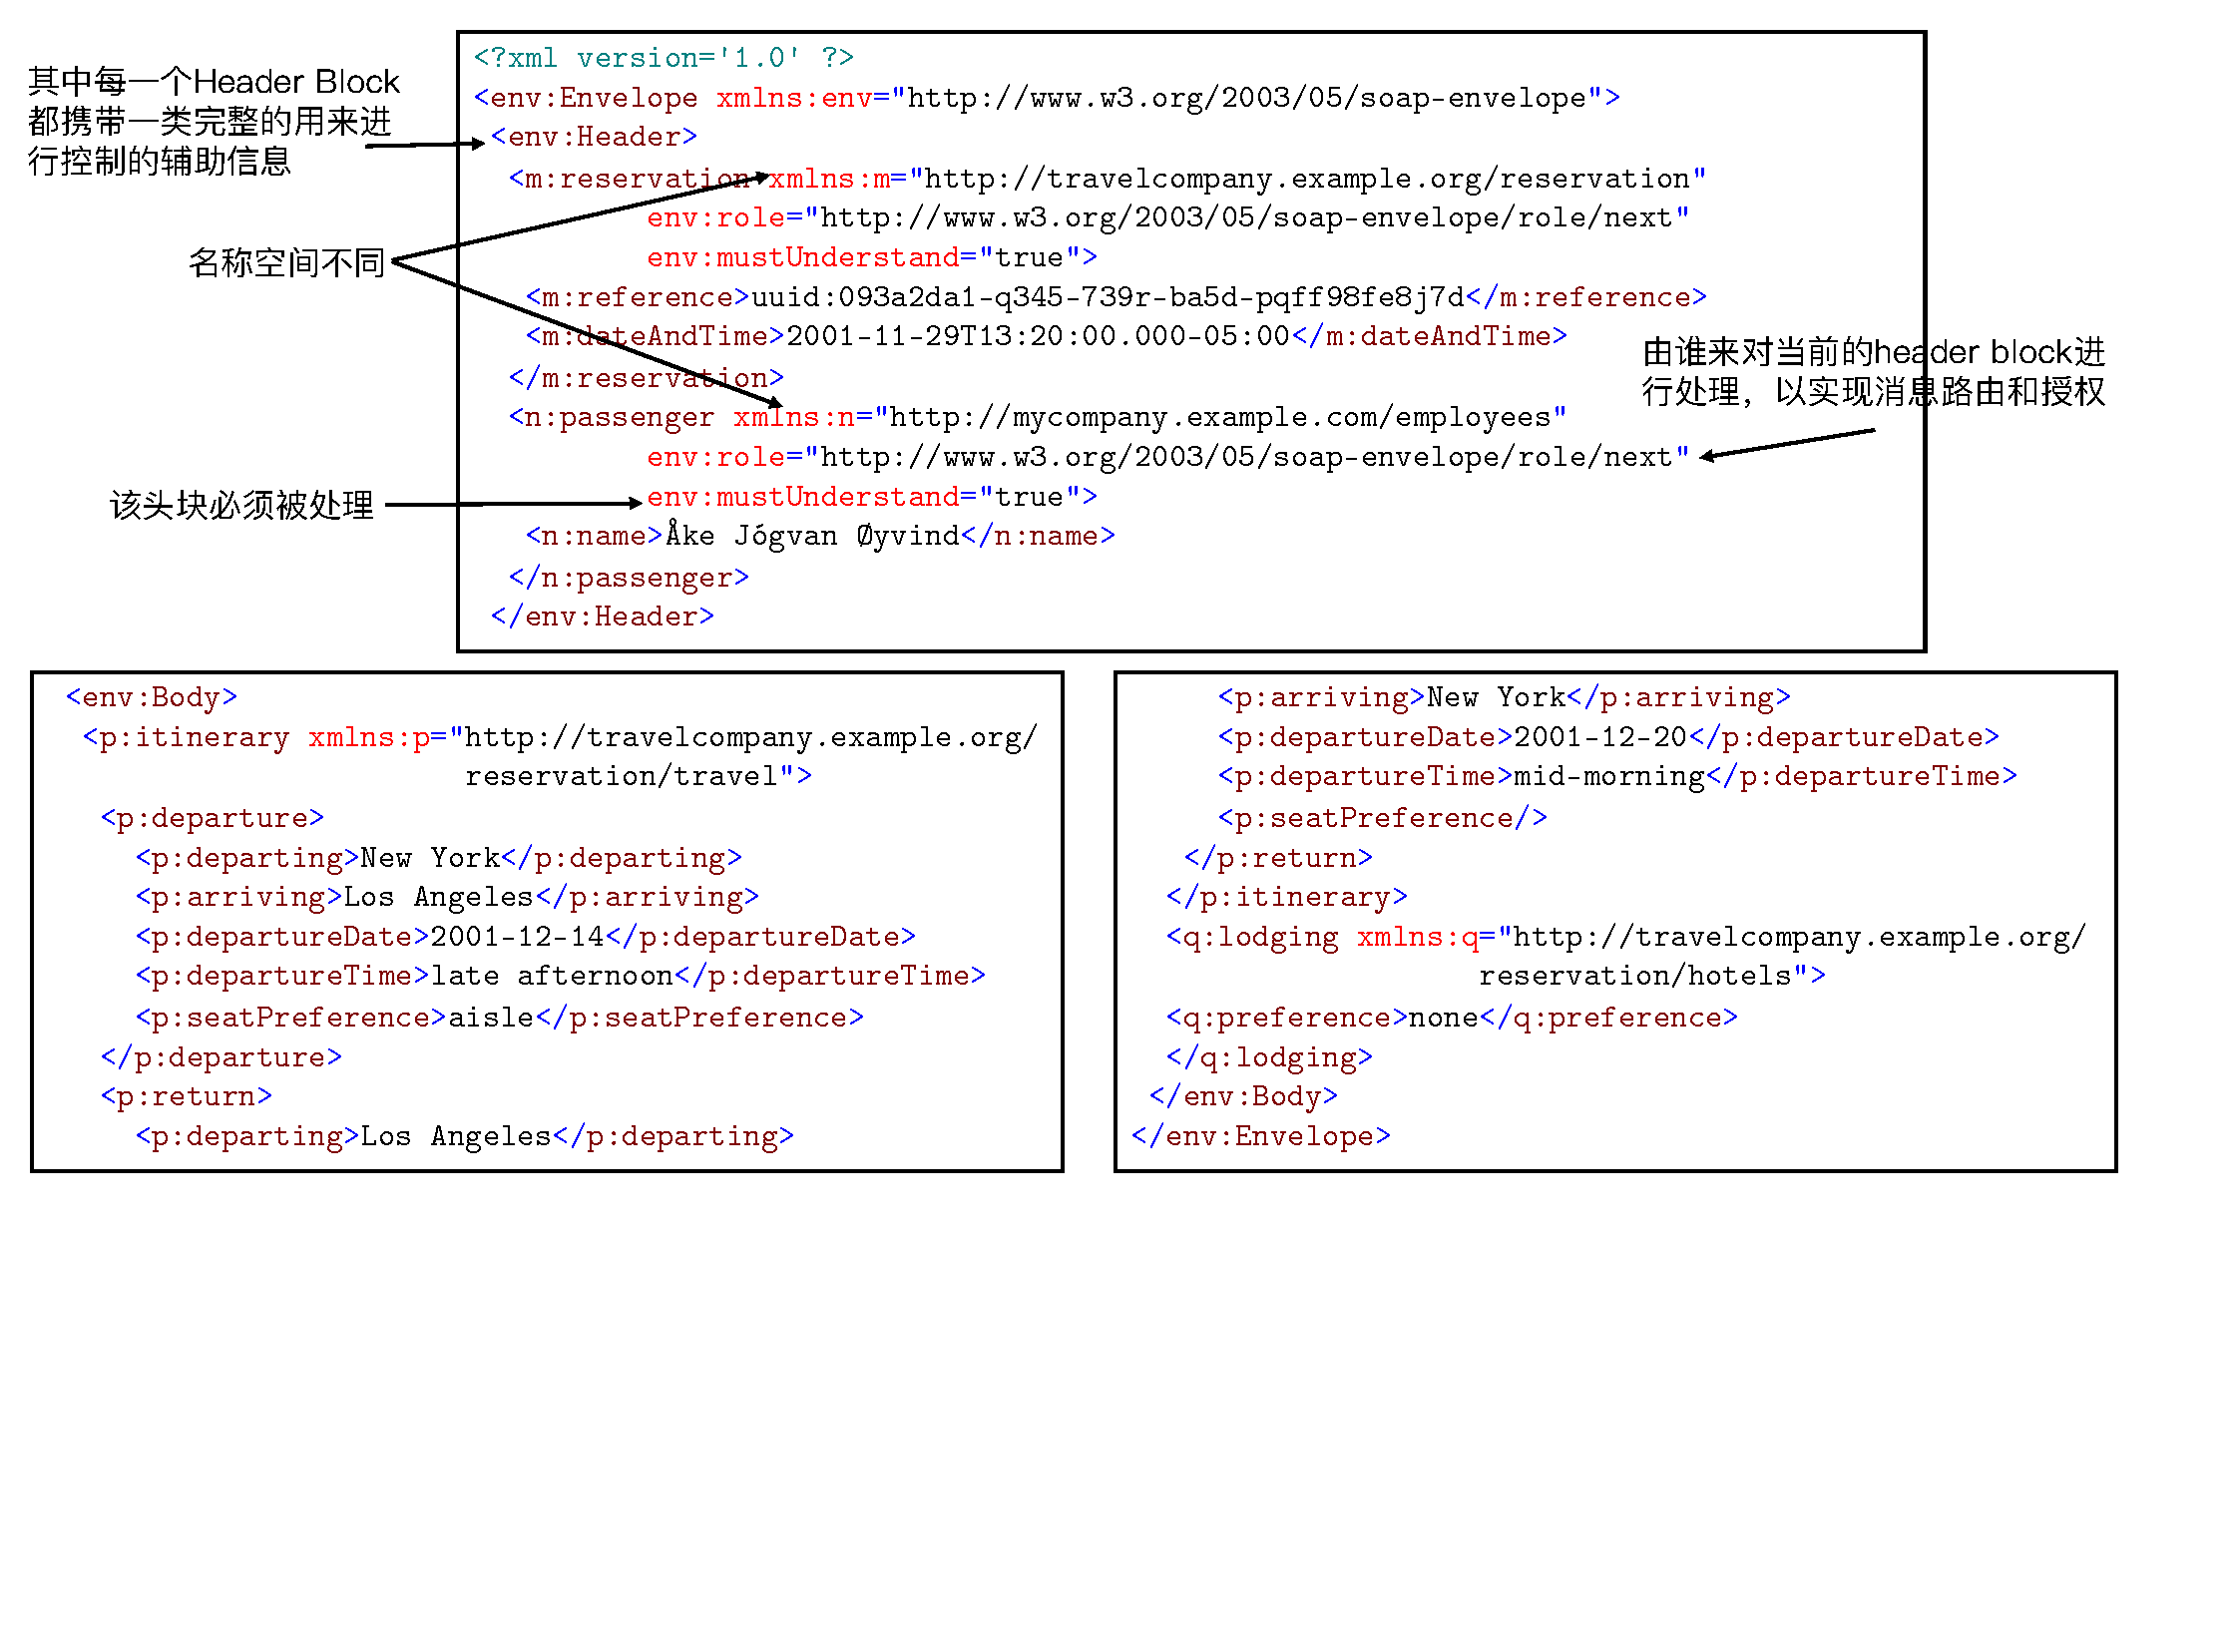
\includegraphics[width=\textwidth]{images/SOAP Messages Example.pdf}
    \vspace{-3em}
\end{figure}

\paragraph*{远程过程调用(RPC)}~{} \par
\begin{figure}[H]
    \vspace{-0.5em}
	\centering
	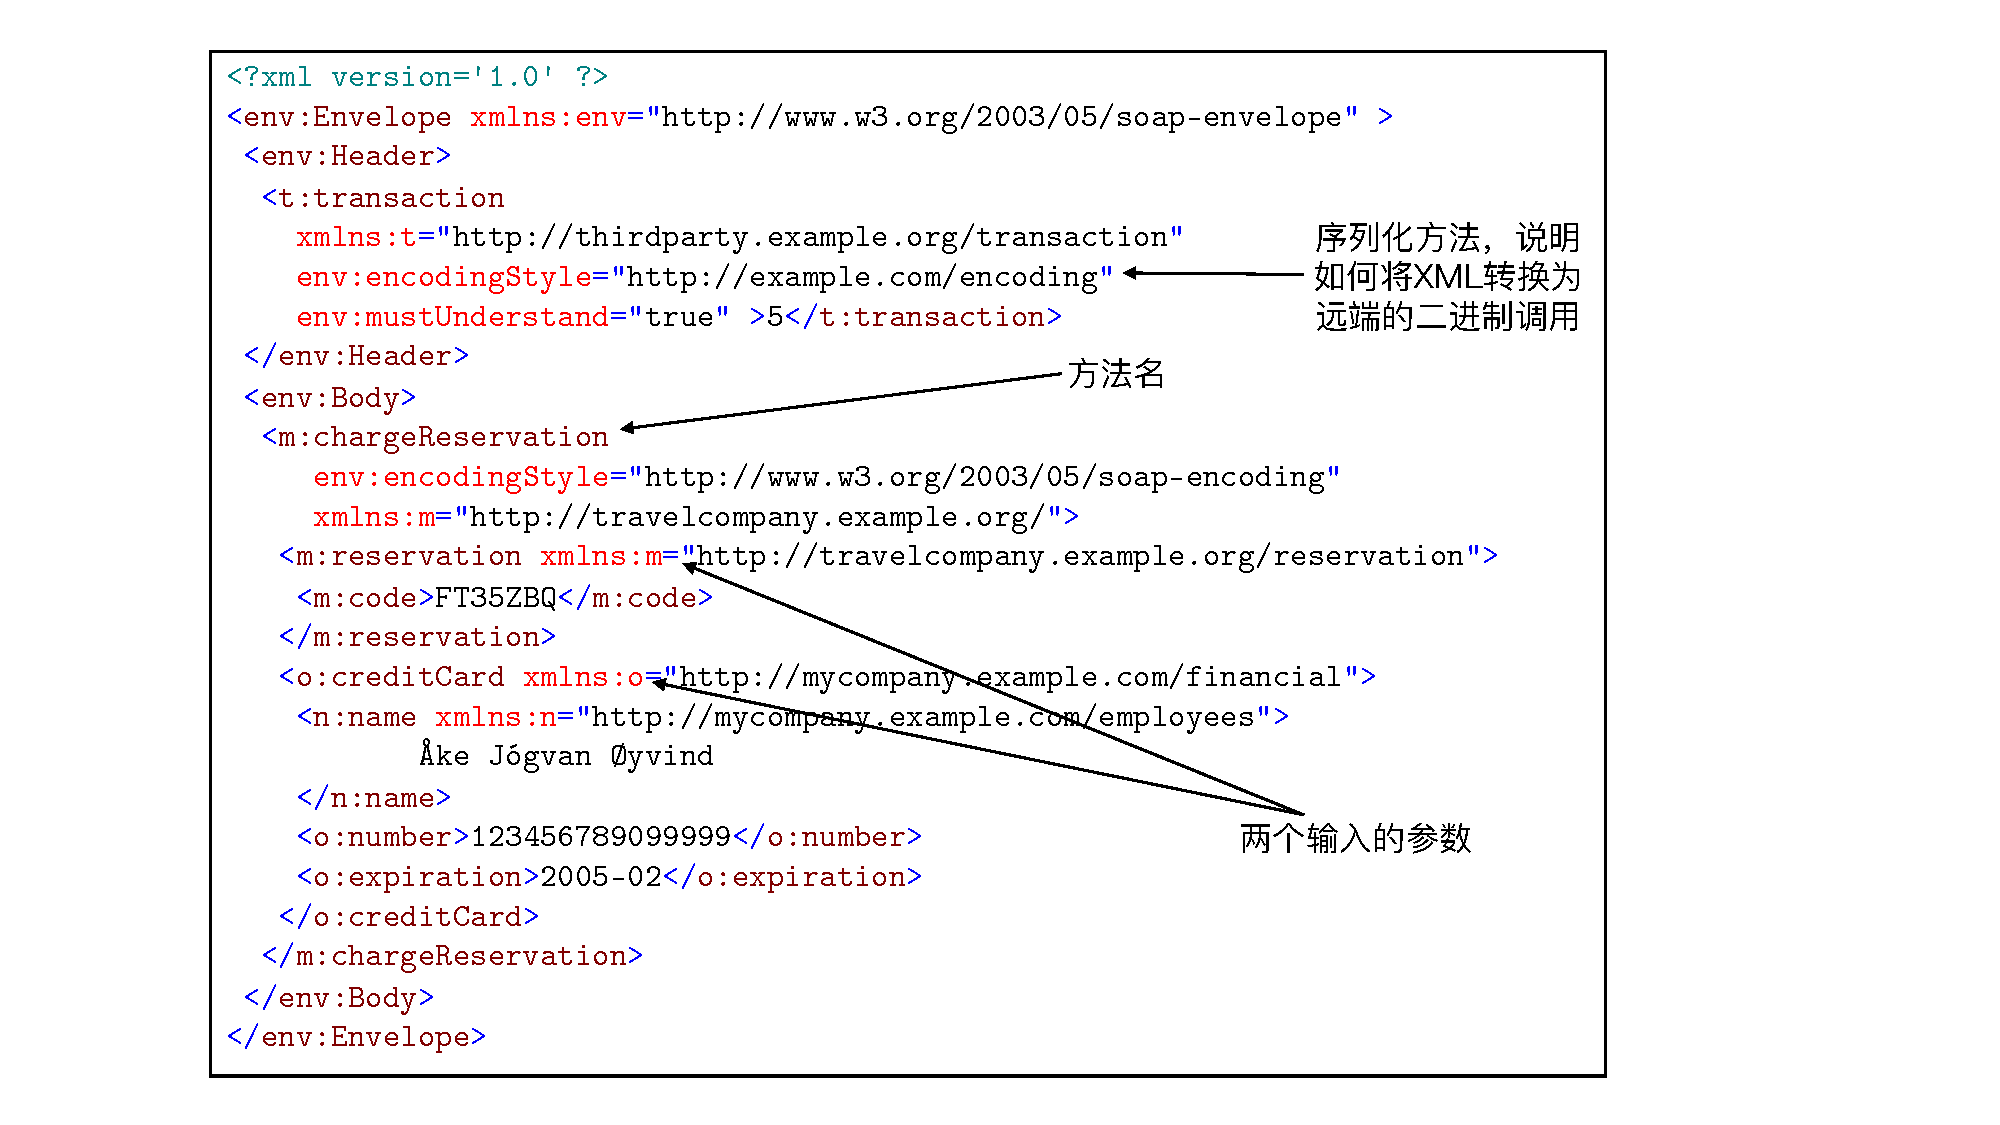
\includegraphics[width=0.67\textwidth]{images/Remote Procedure Calls.pdf}
    \vspace{-2em}
\end{figure}

RPC应答1
\begin{figure}[H]
    \vspace{-0.5em}
	\centering
	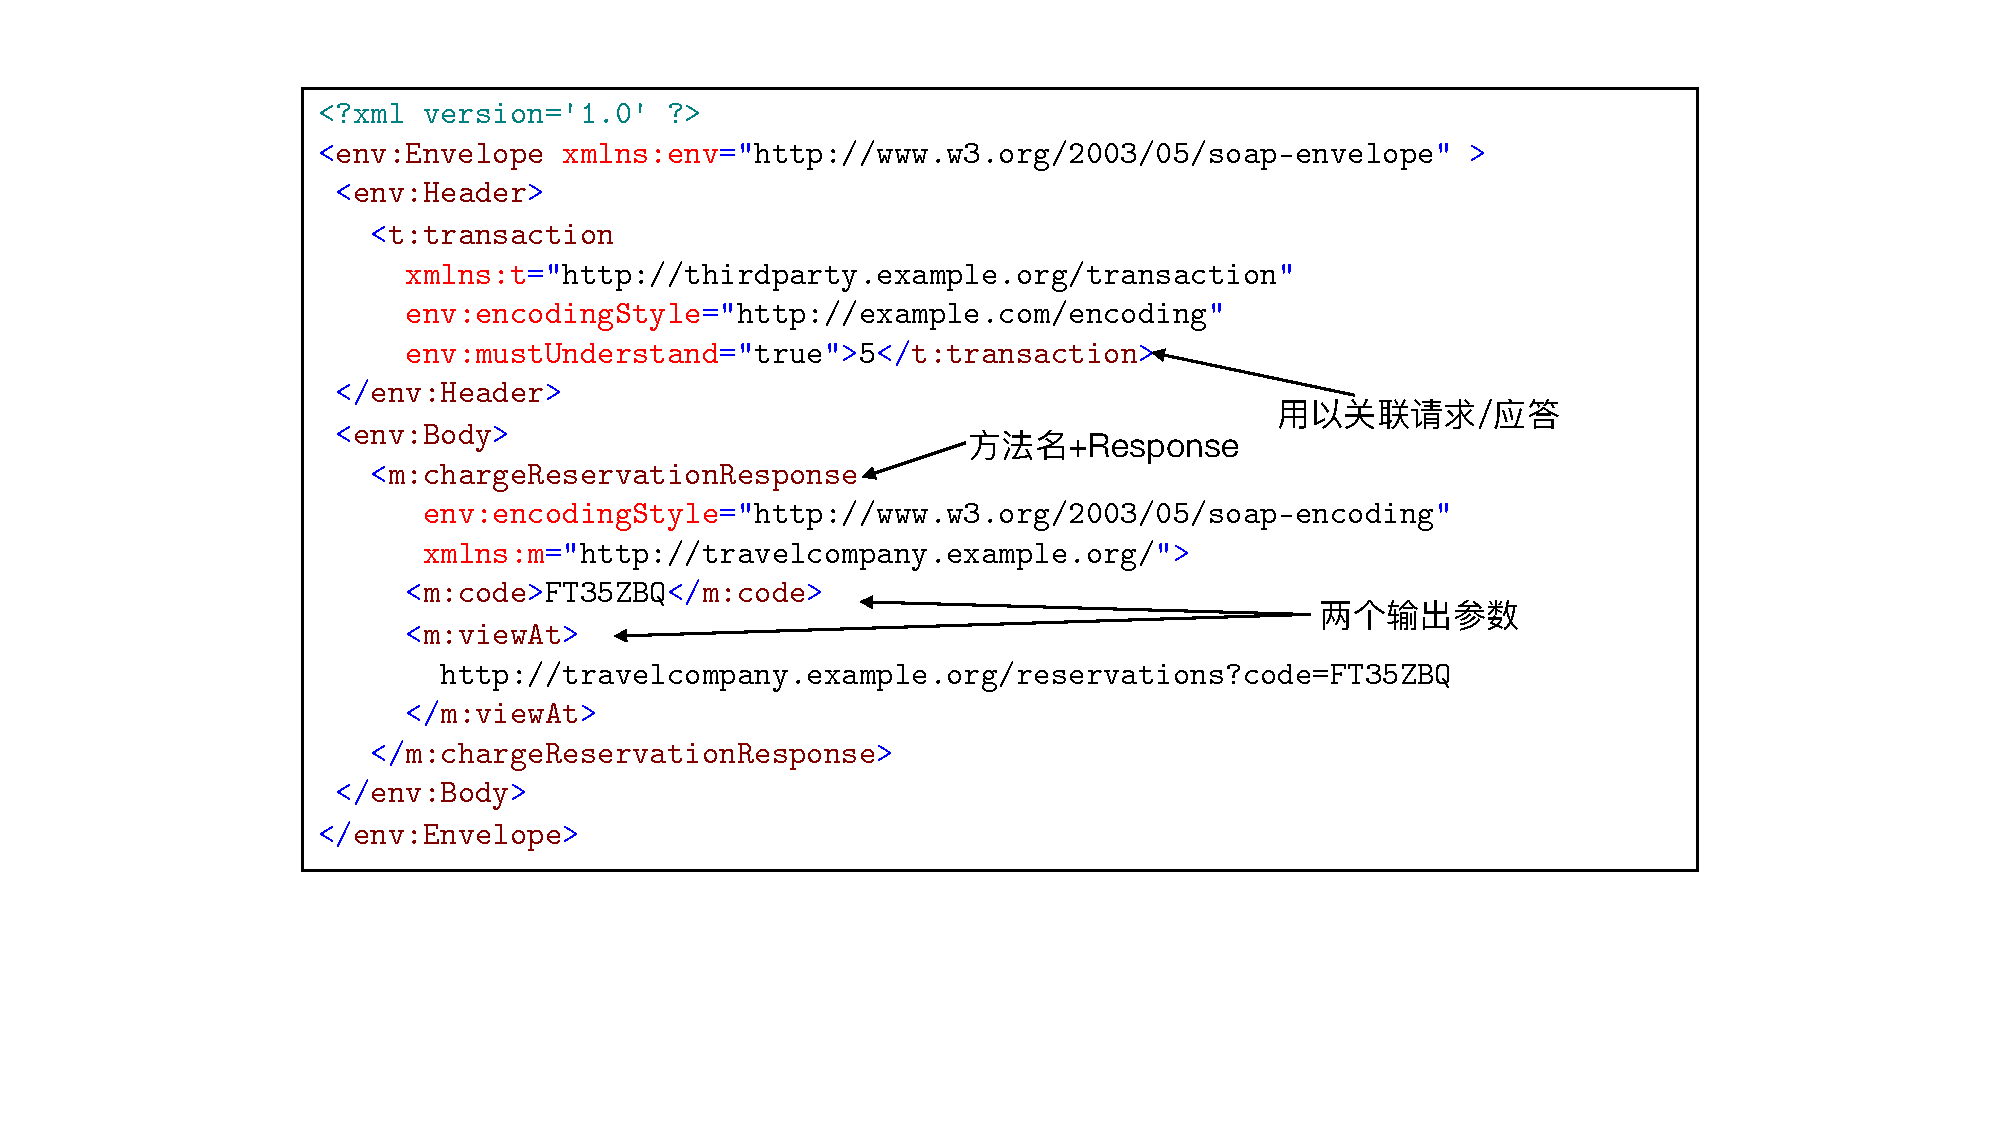
\includegraphics[width=0.75\textwidth]{images/RPC1.pdf}
    \vspace{-1em}
\end{figure}

RPC应答2
\begin{figure}[H]
    \vspace{-0.5em}
	\centering
	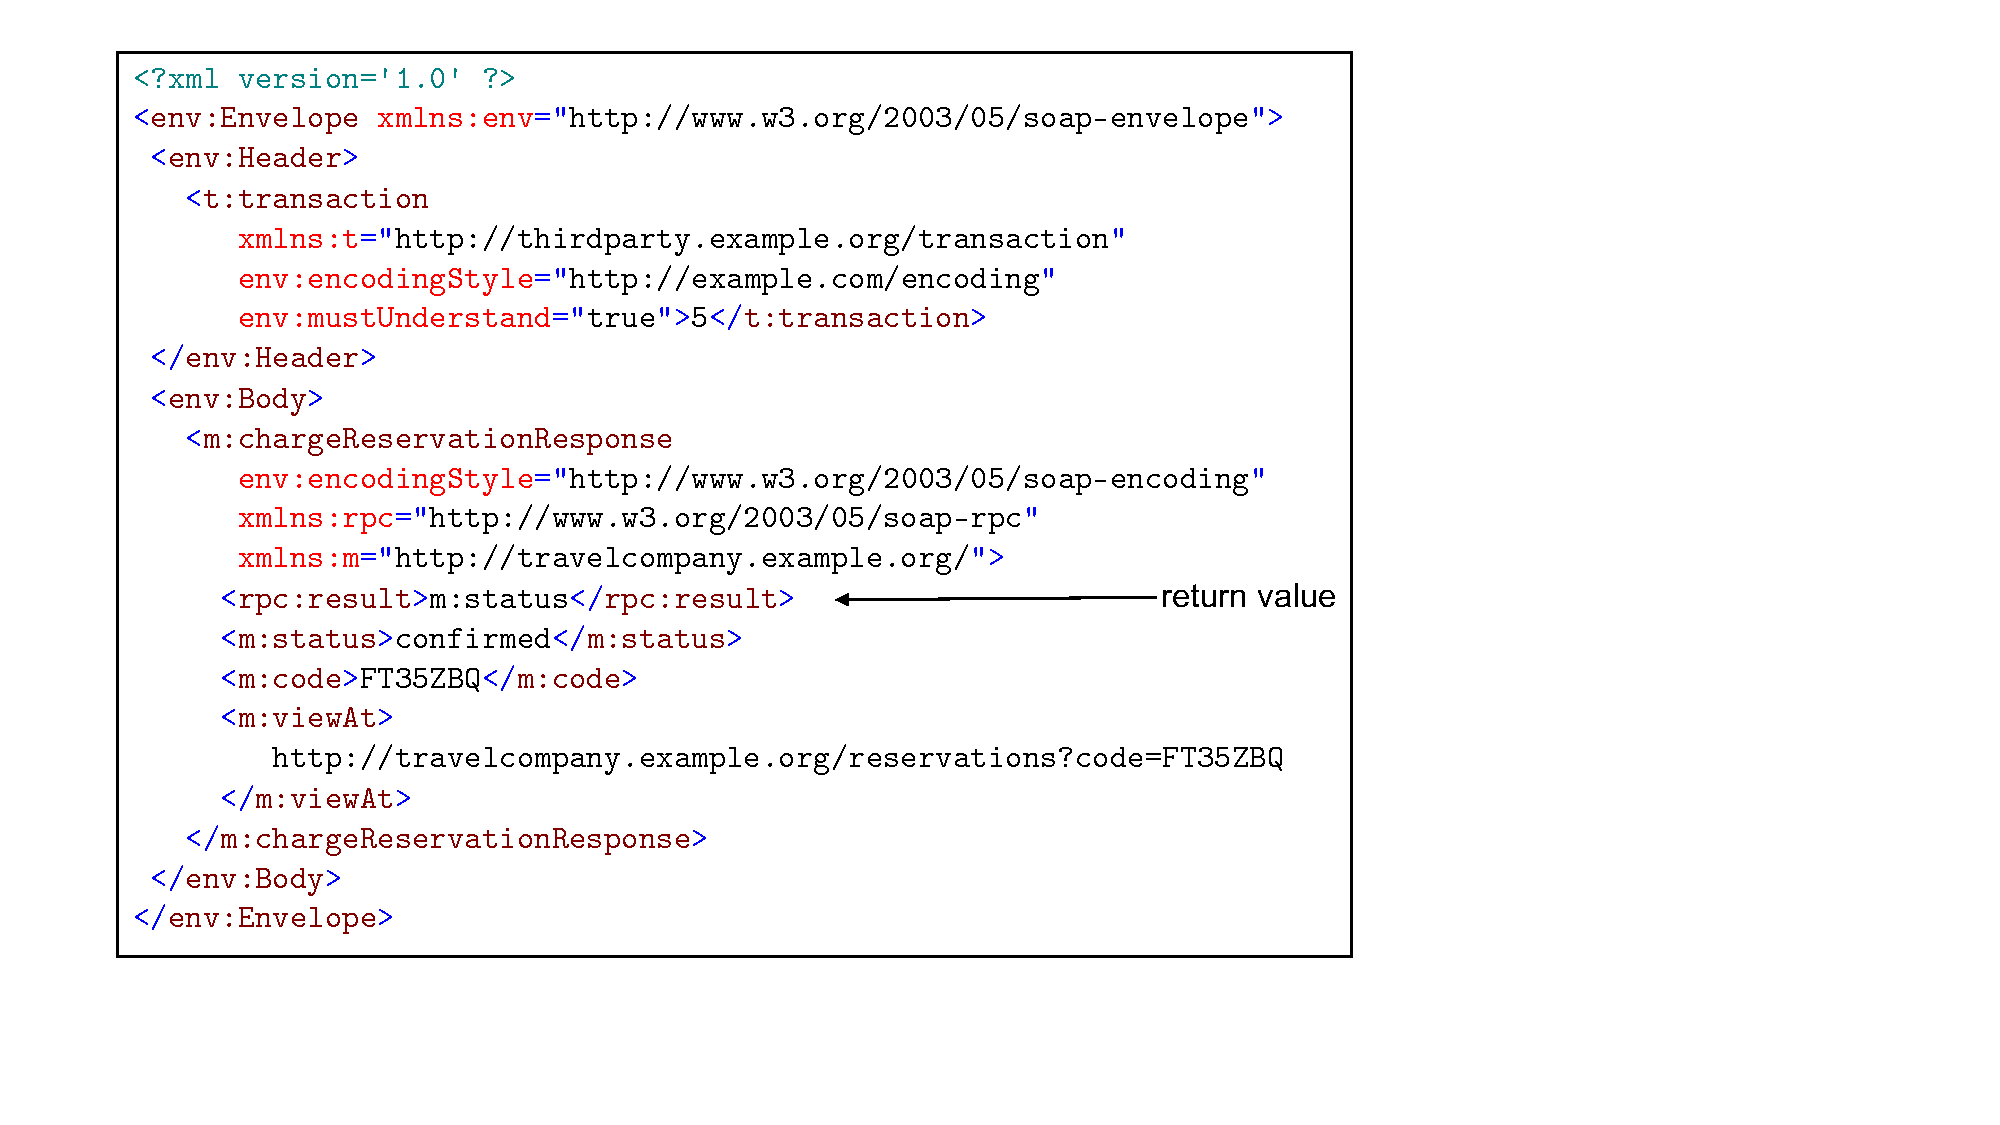
\includegraphics[width=0.7\textwidth]{images/RPC2.pdf}
    \vspace{-1em}
\end{figure}

\paragraph*{出错场景}~{} \par
\begin{figure}[H]
    \vspace{-0.5em}
	\centering
	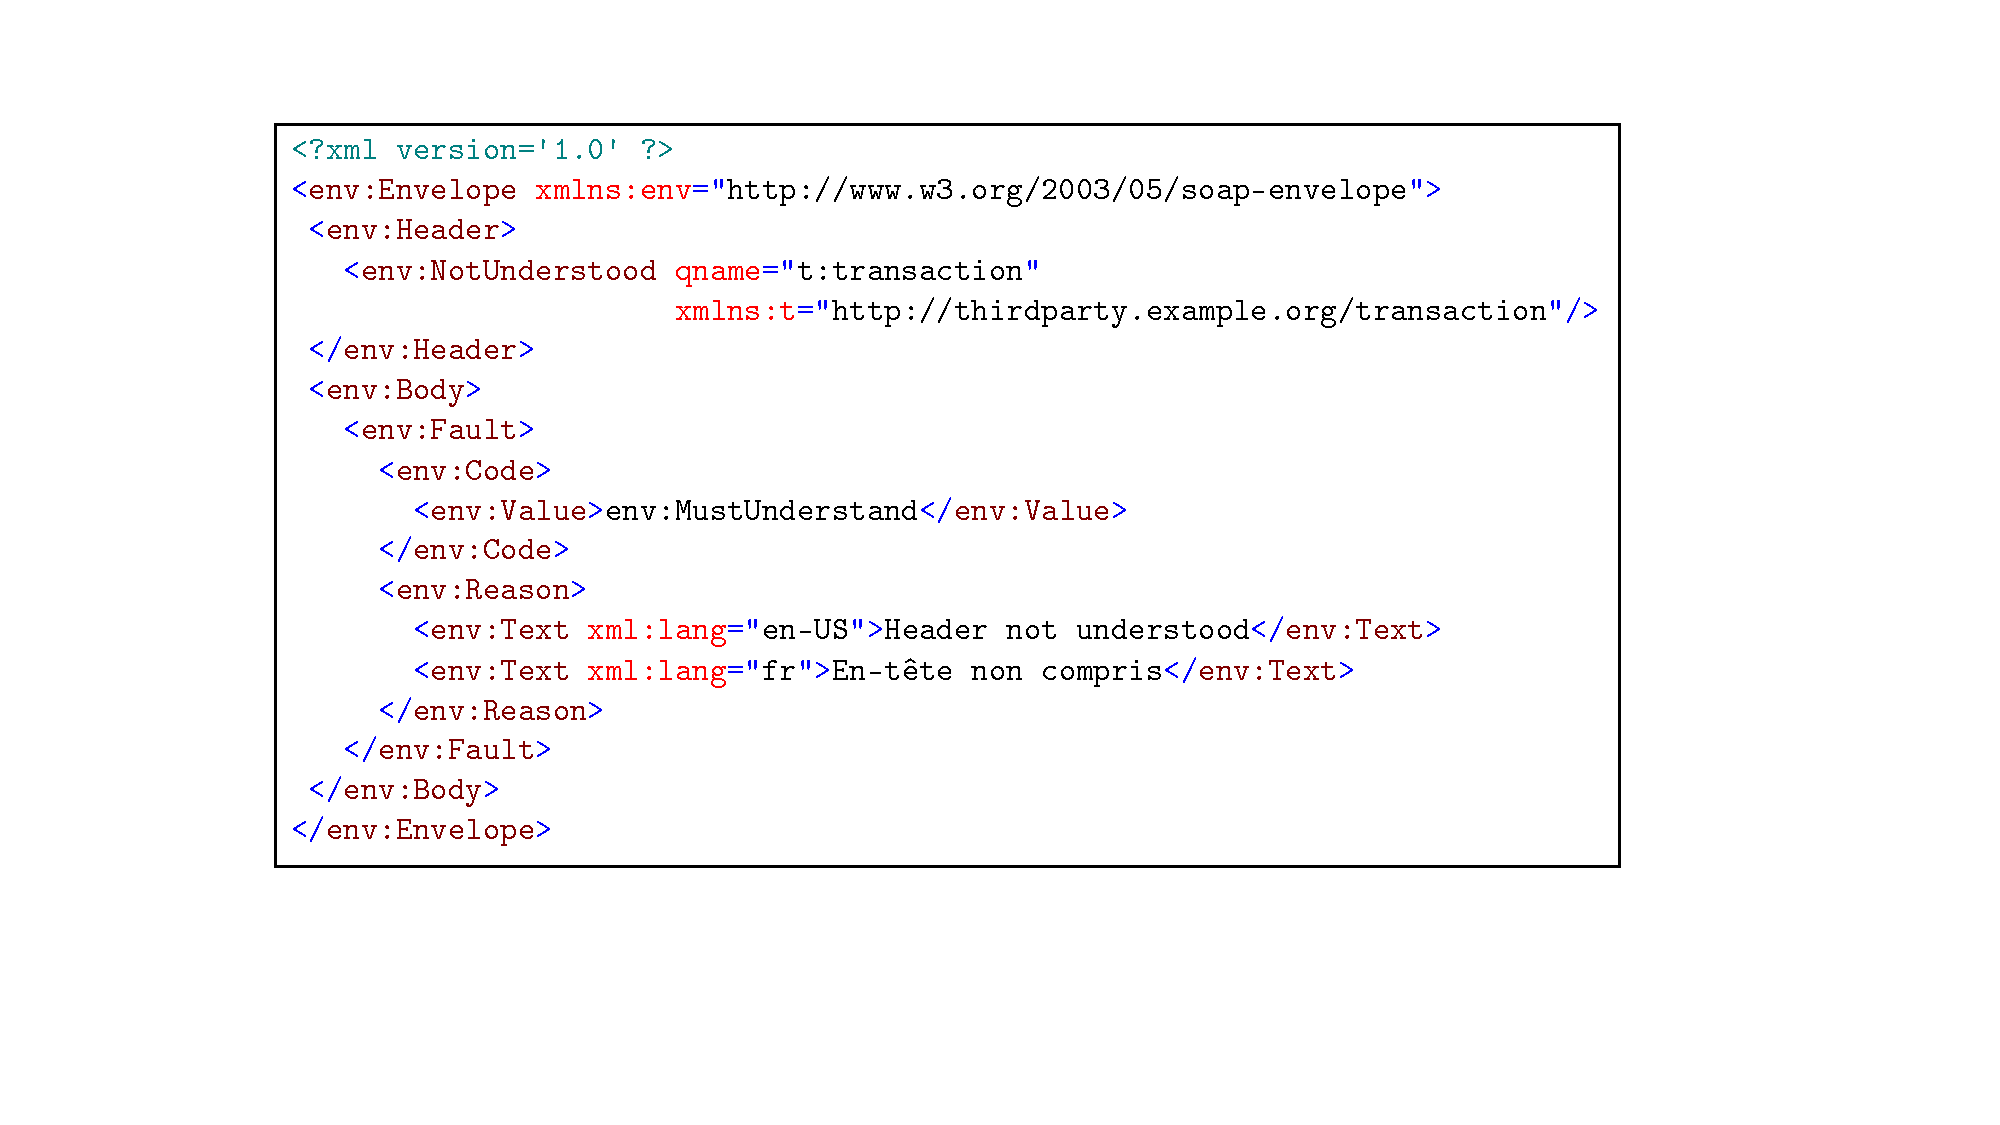
\includegraphics[width=0.75\textwidth]{images/Fault Scenarios.pdf}
    \vspace{-3em}
\end{figure}

\paragraph*{SOAP绑定}~{} \par
在抽象的消息交互框架中,SOAP消息需要使用底层协议完成传输,如何使用底层协议完成 OAP消息的封装、处理和传输,由SOAP绑定进行定义。

最常见的SOAP绑定是HTTP绑定,该绑定使用Web方法(GET和POST),采用HTTP消息交互的方式,支持SOAP消息传递。

此外,它还使用两种消息交换模式(MEP, message exchange patterns),提供了两种通过HTTP交换SOAP消息的方法:
\begin{itemize}
    \item 一种是使用HTTP POST方法在HTTP请求和响应消息的正文中传递SOAP消息,这种方法使用了一个称为SOAP请求-响应MEP的功能
    \item 另一种是使用HTTP GET方法在HTTP请求中返回一个包含SOAP消息的HTTP响应的正文,这种方法使用了一个称为SOAP响应MEP的功能
\end{itemize}

SOAP HTTP POST
\begin{figure}[H]
    \vspace{-0.5em}
	\centering
	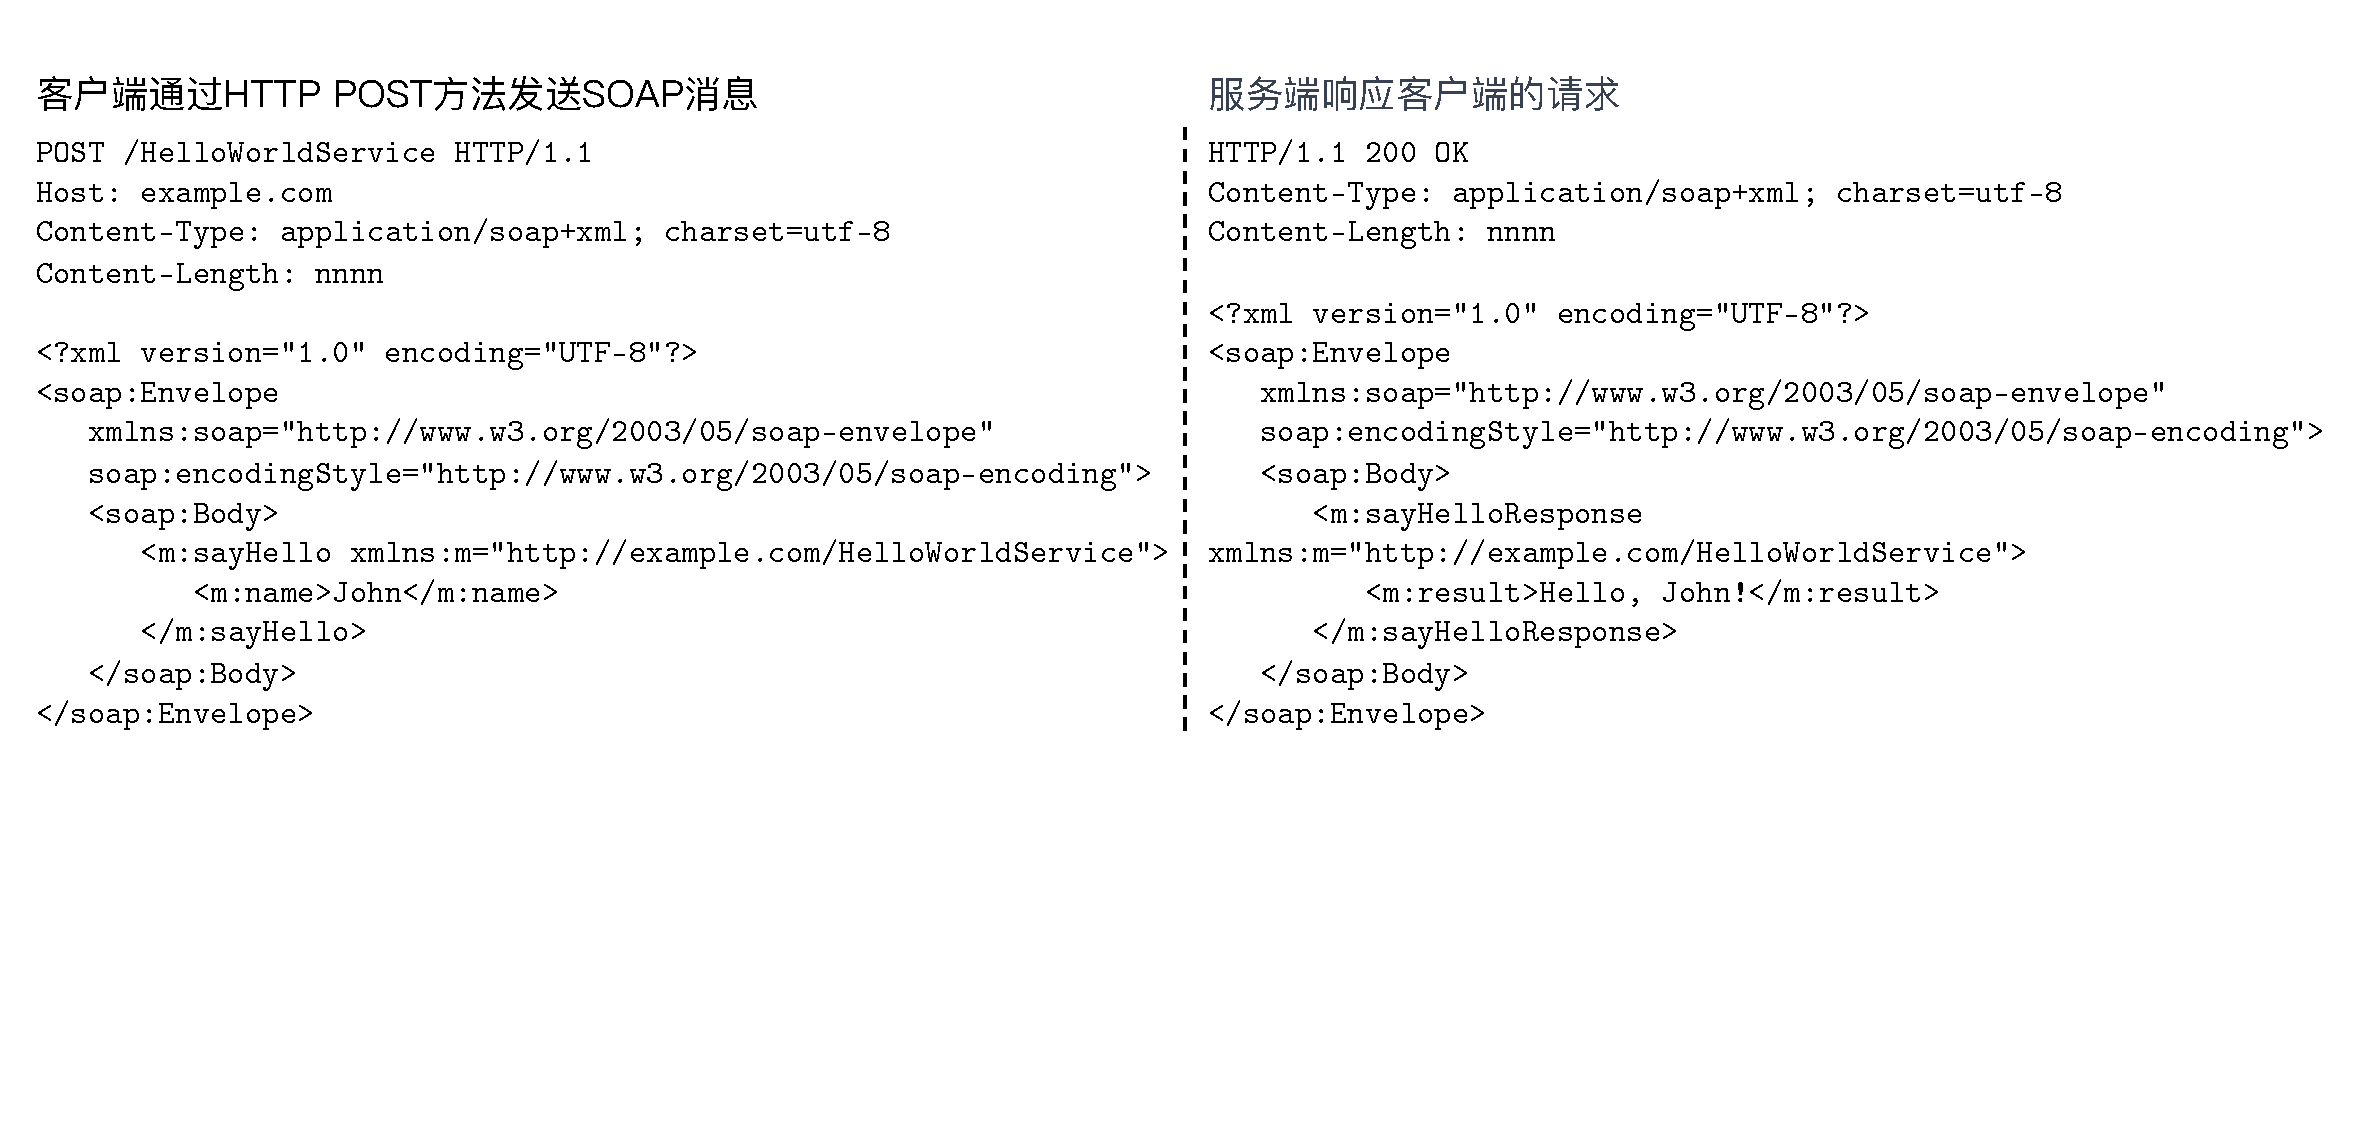
\includegraphics[width=\textwidth]{images/SOAP绑定POST.pdf}
    \vspace{-3em}
\end{figure}

SOAP HTTP GET
\begin{figure}[H]
    \vspace{-0.5em}
	\centering
	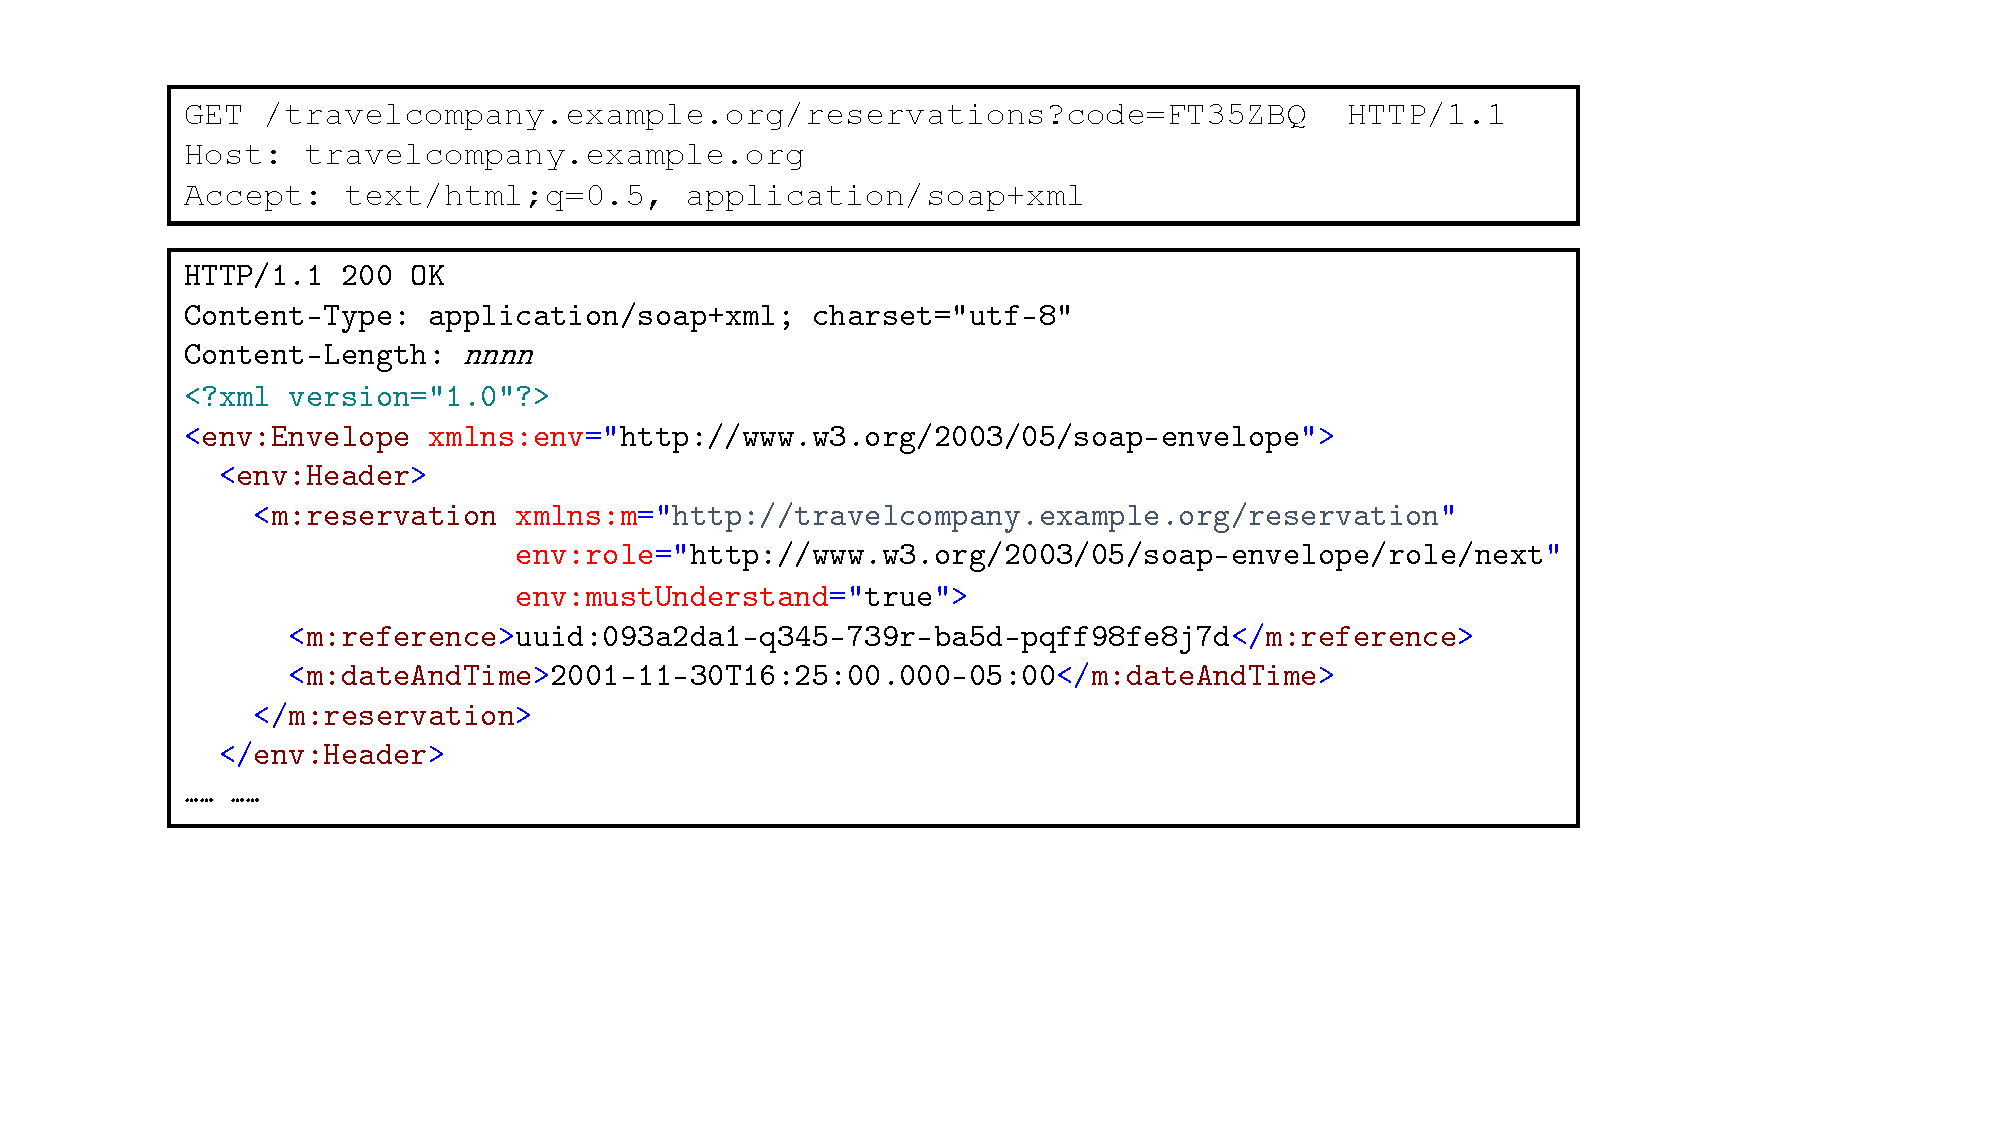
\includegraphics[width=0.8\textwidth]{images/SOAP绑定get.pdf}
    \vspace{-1.5em}
\end{figure}

除了HTTP绑定,其他绑定还可以有SMTP、HTTPS、MIME等

\subsection{WSDL}

\subsubsection{WSDL的引入}
\begin{itemize}
    \item 现在我们有:
    \begin{itemize}
        \item XML,Namespace,XML Schema完成消息格式和数据结构定义
        \item SOAP作为传递XML消息的传输协议(最简)
    \end{itemize}
    \item 下一个问题是:我们怎么知道,在什么地方/以什么方式/能够调用到什么样的Web Service?
    \begin{itemize}
        \item 一个可能的方法是,Out-of-band(例如完成了一个Web Service开发后通过邮件告诉相应的人有关信息或直接提供相关说明文档)
        \item 为什么使用WSDL:提供了一种基于XML的标准接口定义语言/服务能力定义语言,用以在服务的提供者/调用者/服务注册之间,交换必要的有关Web Service 的信息
        \item WSDL是否携带了关于Web Service的足够信息?可能是也可能否,取决于Web Service本身的复杂性和业务特性
    \end{itemize}
\end{itemize}

\subsubsection{WSDL模型的基本概念}
WSDL是用以描述网络服务的XML格式,它将服务描述为基于消息(面向文档/面向过程)运作的端点(endpoints)集合。通常WSDL、SOAP 和 XML Schema 会被同时使用。
\vspace{-0.5em}
\begin{spacing}{1.2}
    \begin{longtable}{|m{4cm}|m{9cm}|}
        \hline
        \multicolumn{1}{|c|}{WSDL回答了}  &  \multicolumn{1}{c|}{WSDL提供了}\\ \hline
        \vspace{-1.3em}
        \begin{itemize}[leftmargin=1.5em,itemsep=-2pt]
            \item 服务用来干什么
            \item 服务在哪
            \item 如何调用服务
            \vspace{-1.5em}
        \end{itemize} &  
        \vspace{-1.3em}
        \begin{itemize}[leftmargin=1.5em,itemsep=-2pt]
            \item 功能信息
            \item 消息结构(如何说明消息交互中的数据类型)
            \item 协议绑定(如何将抽象消息映射为具体的网络传输)
            \vspace{-1.5em}
        \end{itemize}
        \\\hline
    \end{longtable}
\end{spacing}
\vspace{-1em}

WSDL的历史
\begin{itemize}
    \item WSDL 1.0(2000年9月)由IBM,Microsoft和Ariba开发,用于描述其SOAP工具包的Web服务。它是通过将IBM的NASSL(网络应用程序服务规范语言)和Microsoft的SDL(服务描述语言)两种服务描述语言结合而构建的。
    \item WSDL 1.1于2001年3月发布,是对WSDL 1.0的正式规范化。在1.0和1.1间没有引入重大变化。
    \item WSDL 1.2(2003年6月)是W3C的工作草案,后因与WSDL 1.1有重大差异更名为WSDL 2.0。
    \begin{itemize}
        \item 根据W3C的说法,WSDL 1.2比以前的版本更易于开发人员使用和更加灵活。WSDL 1.2试图删除不可互操作的特性,并更好地定义了HTTP 1.1绑定。
        \item 大多数SOAP服务器/供应商不支持WSDL 1.2。
    \end{itemize}
    \item WSDL 2.0于2007年6月成为W3C推荐标准。
\end{itemize}

\subsubsection{WSDL 2.0信息集结构}
\begin{figure}[H]
    \vspace{-1em}
	\centering
	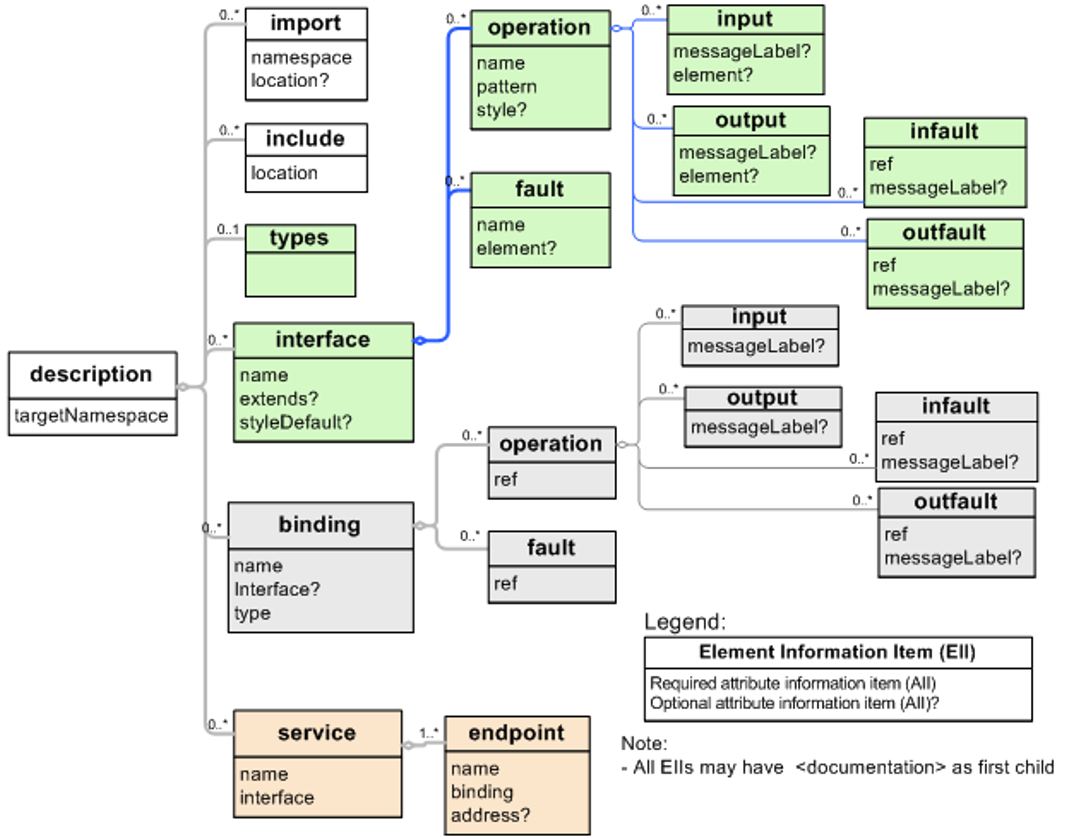
\includegraphics[width=0.6\textwidth]{images/WSDL 2.0信息集结构.png}
    \vspace{-2.5em}
\end{figure}

\begin{itemize}
    \item import、include:主要用来对于撰写在多个文档中间的 WSDL 信息进行拼接,前者用于从不同的名称空间引入,后者用于从相同的名称空间引入
    \item types:用来说明消息结构
    \item interface:用来指定抽象意义下服务所提供的能力的相关接口
    \item binding:用来将 inerface 指定的抽象的消息格式转为具体的消息格式
    \item service:通过聚合 endpoint 在 interface 和 binding 之间来创建映射关系
\end{itemize}

\subsubsection{WSDL 2.0的语法和机制}
\paragraph*{定义声明和名称空间}~{} \par
\begin{figure}[H]
    \vspace{-0.5em}
	\centering
	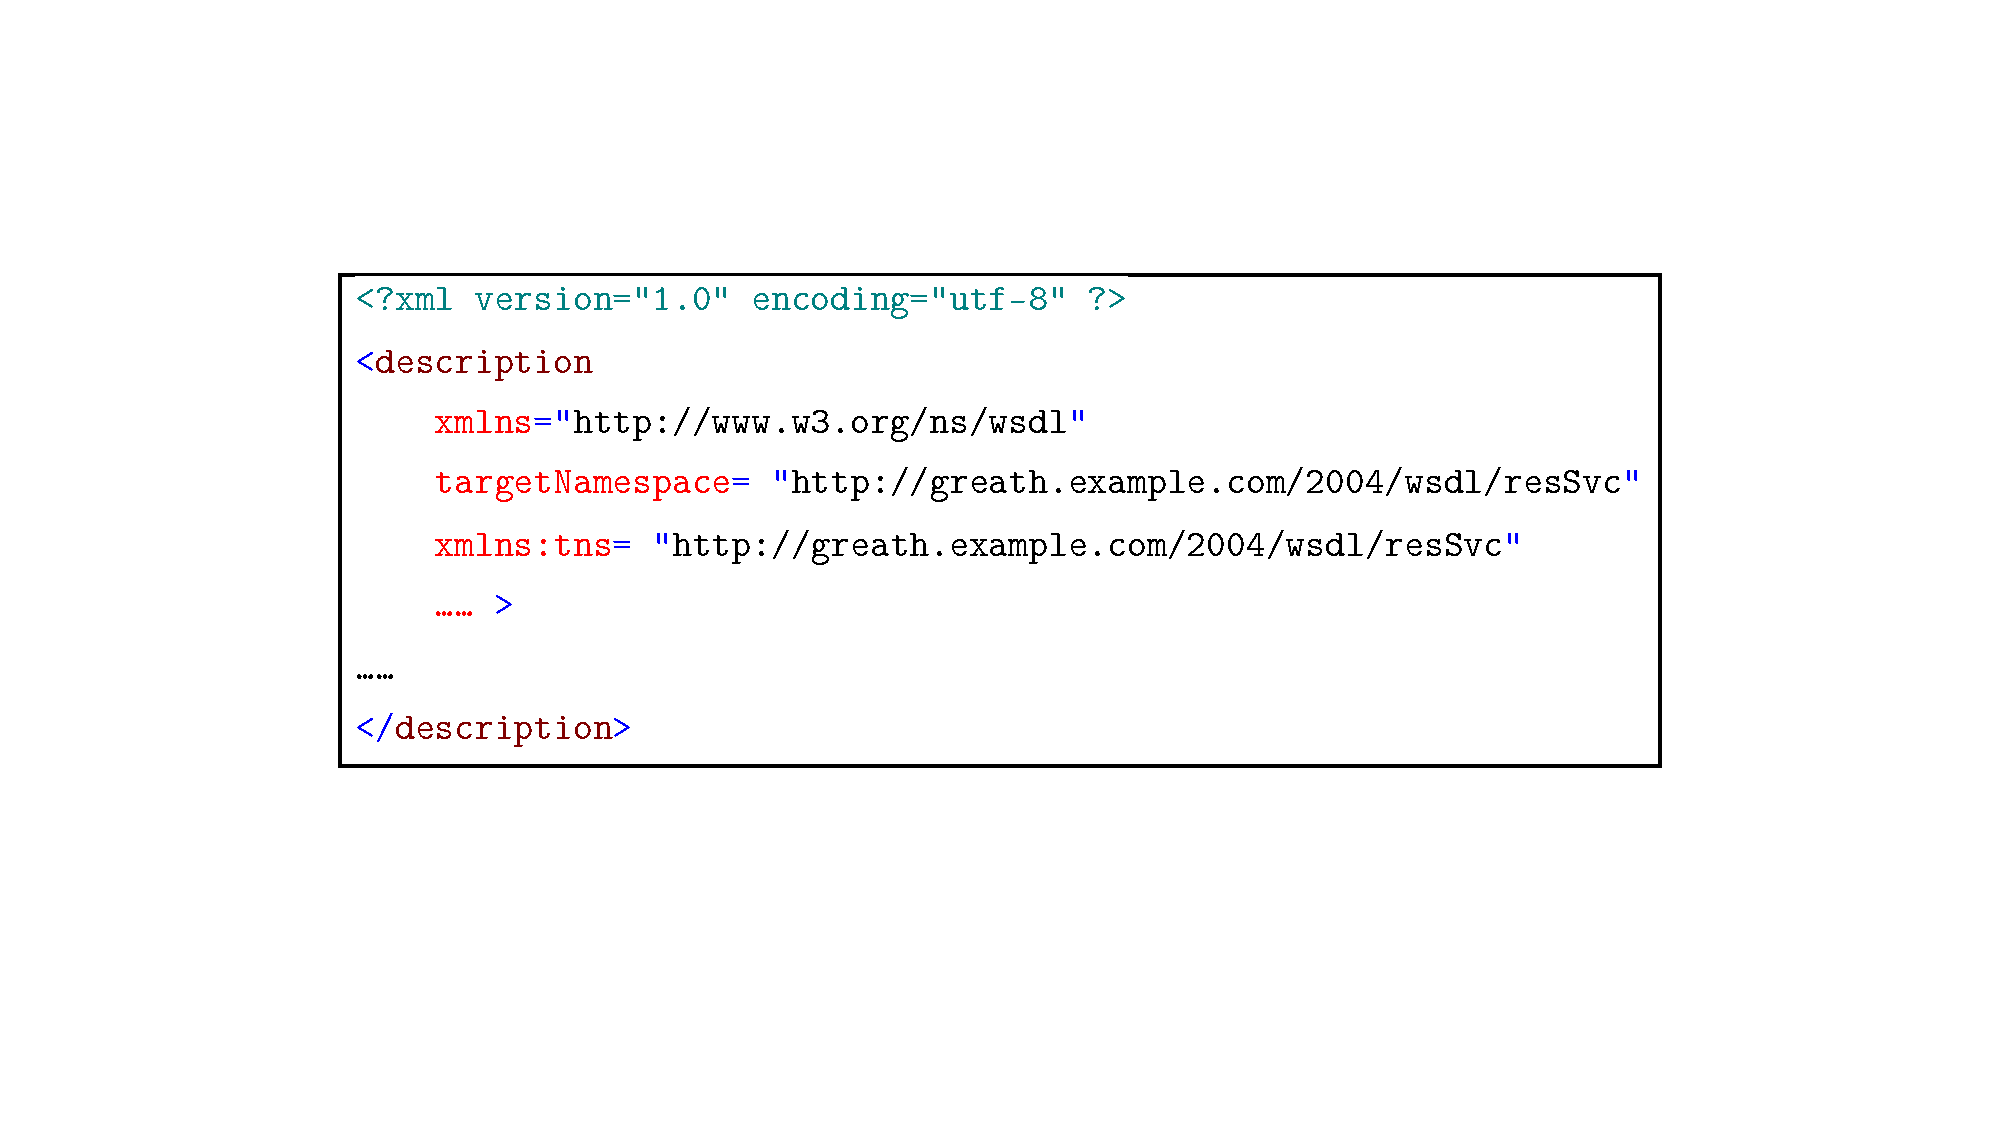
\includegraphics[width=0.65\textwidth]{images/定义声明和名称空间.pdf}
    \vspace{-1.5em}
\end{figure}

\paragraph*{定义消息类型types}~{} \par
\begin{figure}[H]
    \vspace{-0.5em}
	\centering
	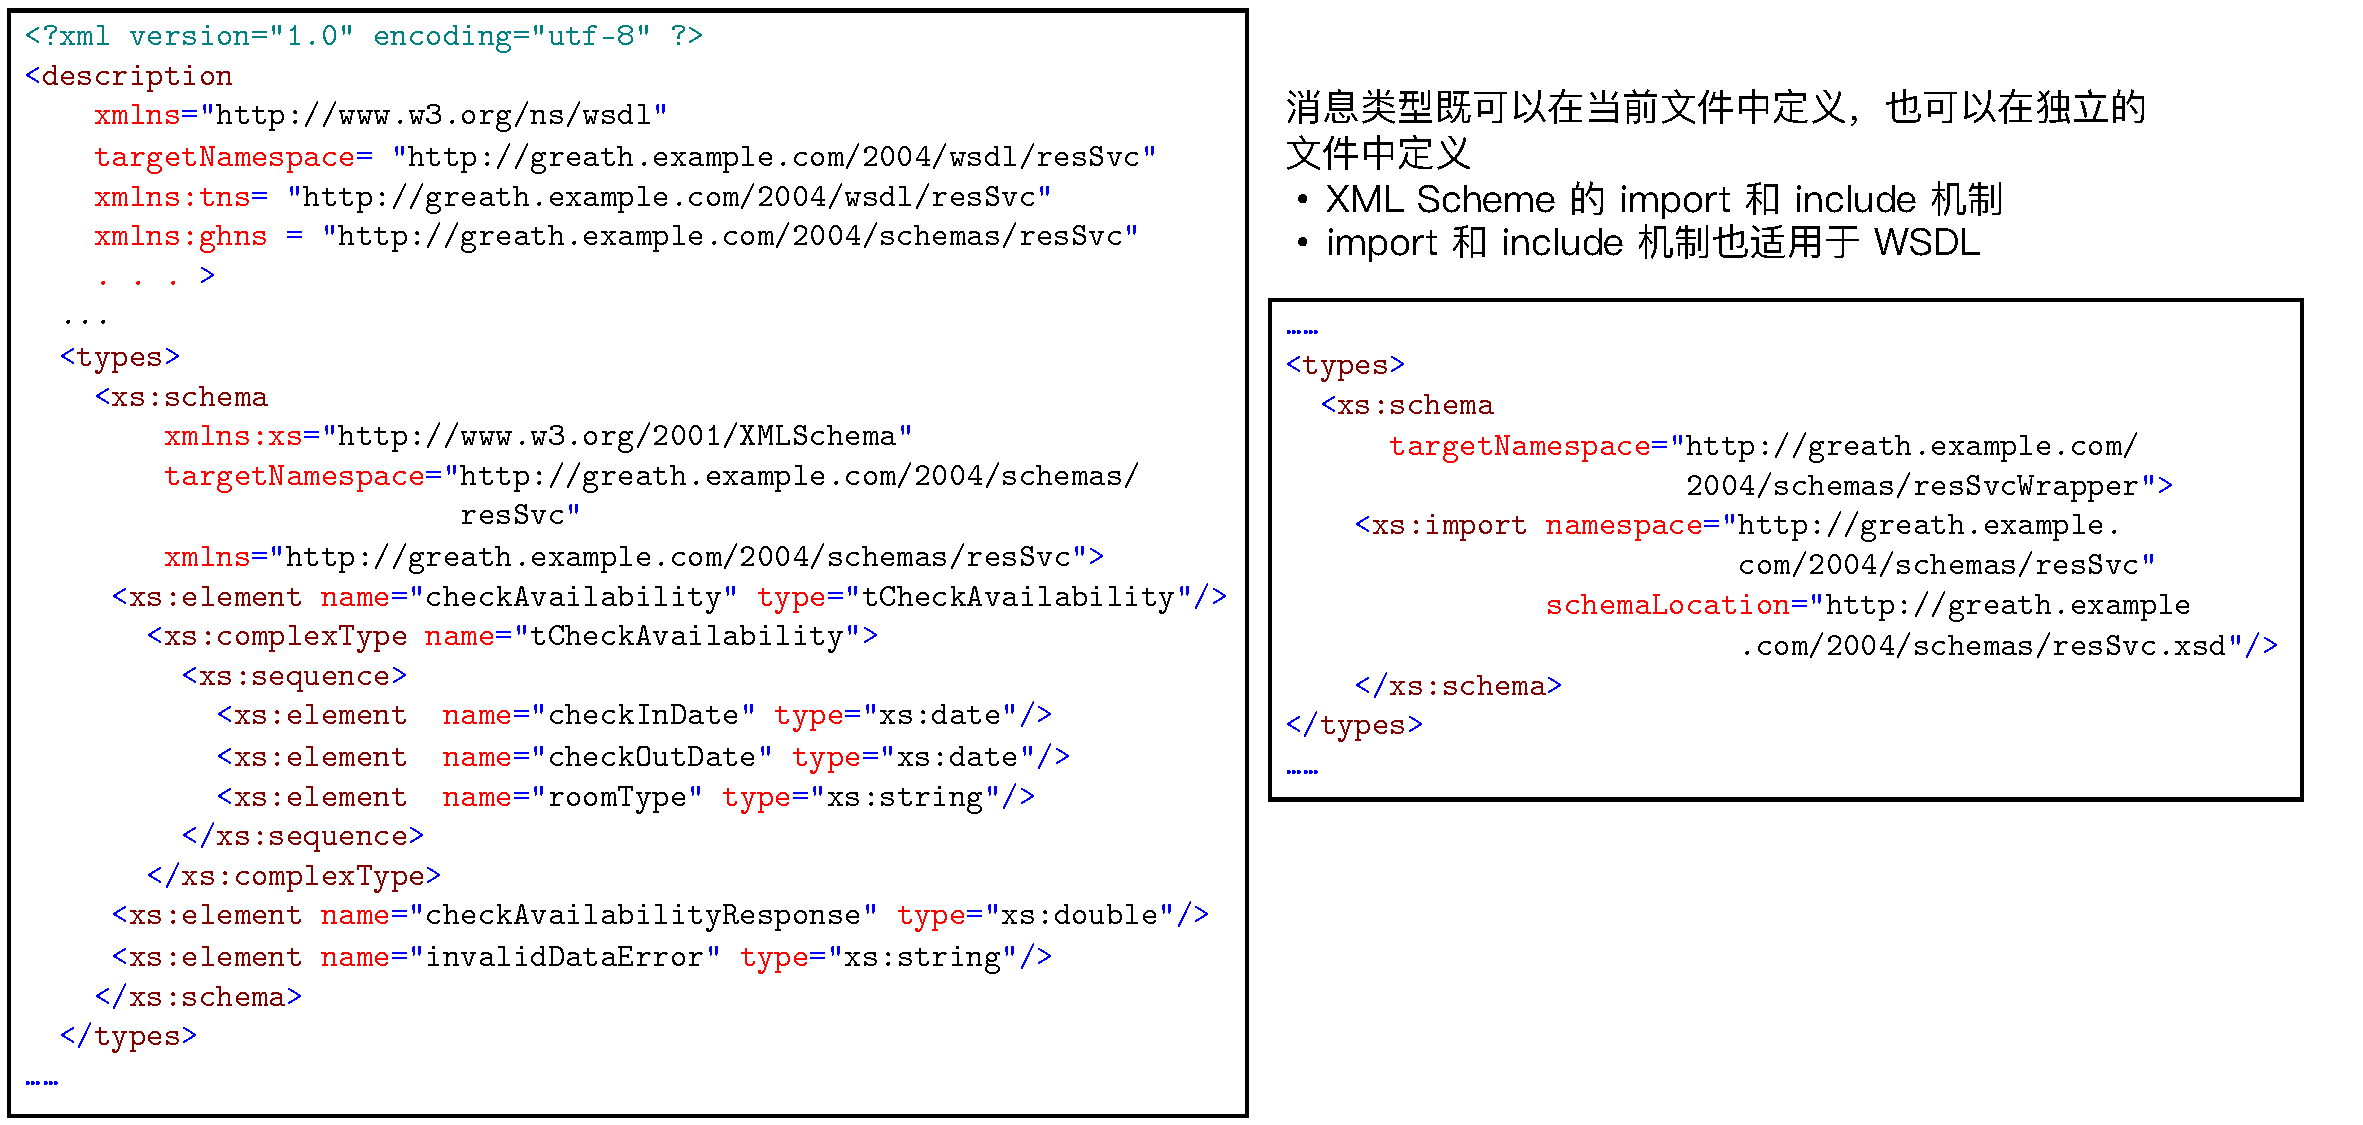
\includegraphics[width=\textwidth]{images/定义消息类型.pdf}
    \vspace{-3em}
\end{figure}

\paragraph*{定义接口interface}~{} \par
\begin{figure}[H]
	\setcounter{subfigure}{0}
	\centering
	\vspace{-1.5em}	
	\subfloat[定义接口interface]{
	\begin{minipage}[t]{0.66\linewidth}
	\centering
	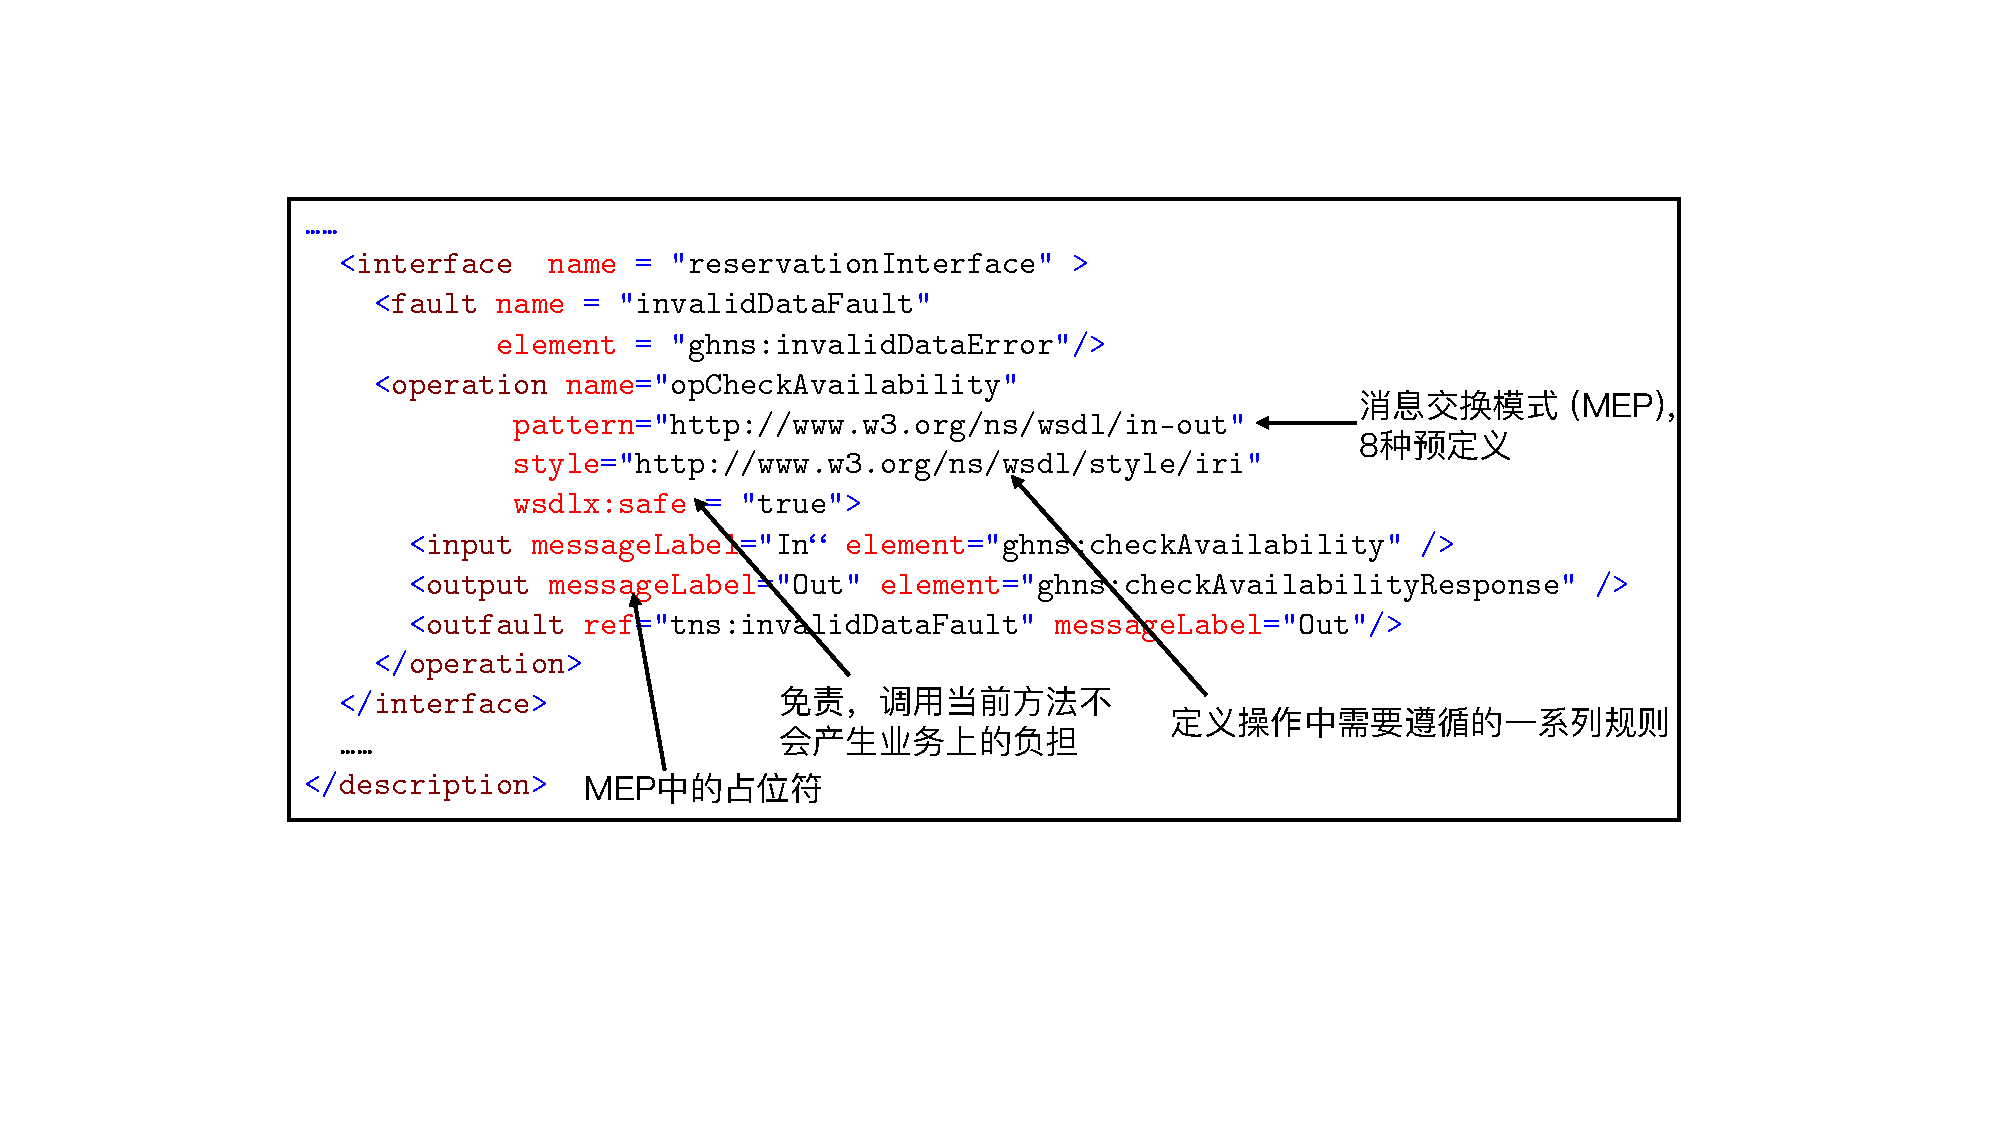
\includegraphics[width=\linewidth]{images/定义接口.pdf}
	\end{minipage}
	}
	\subfloat[4种基本的MEP,若每一种再加上出错处理,就得到另外4种]{
	\begin{minipage}[t]{0.31\linewidth}
	\centering
	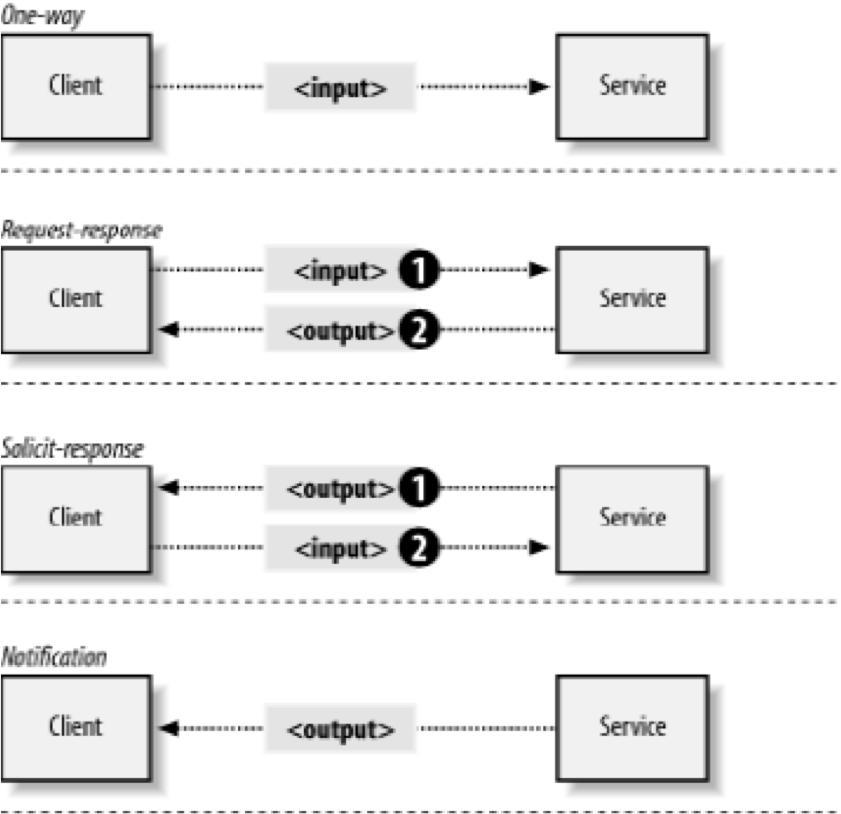
\includegraphics[width=\linewidth]{images/4种基本MEP.png}
	\end{minipage}
	}
	\centering
	\vspace{-4em}
\end{figure}

\paragraph*{定义绑定binding}~{} \par
\begin{figure}[H]
    \vspace{-0.7em}
	\centering
	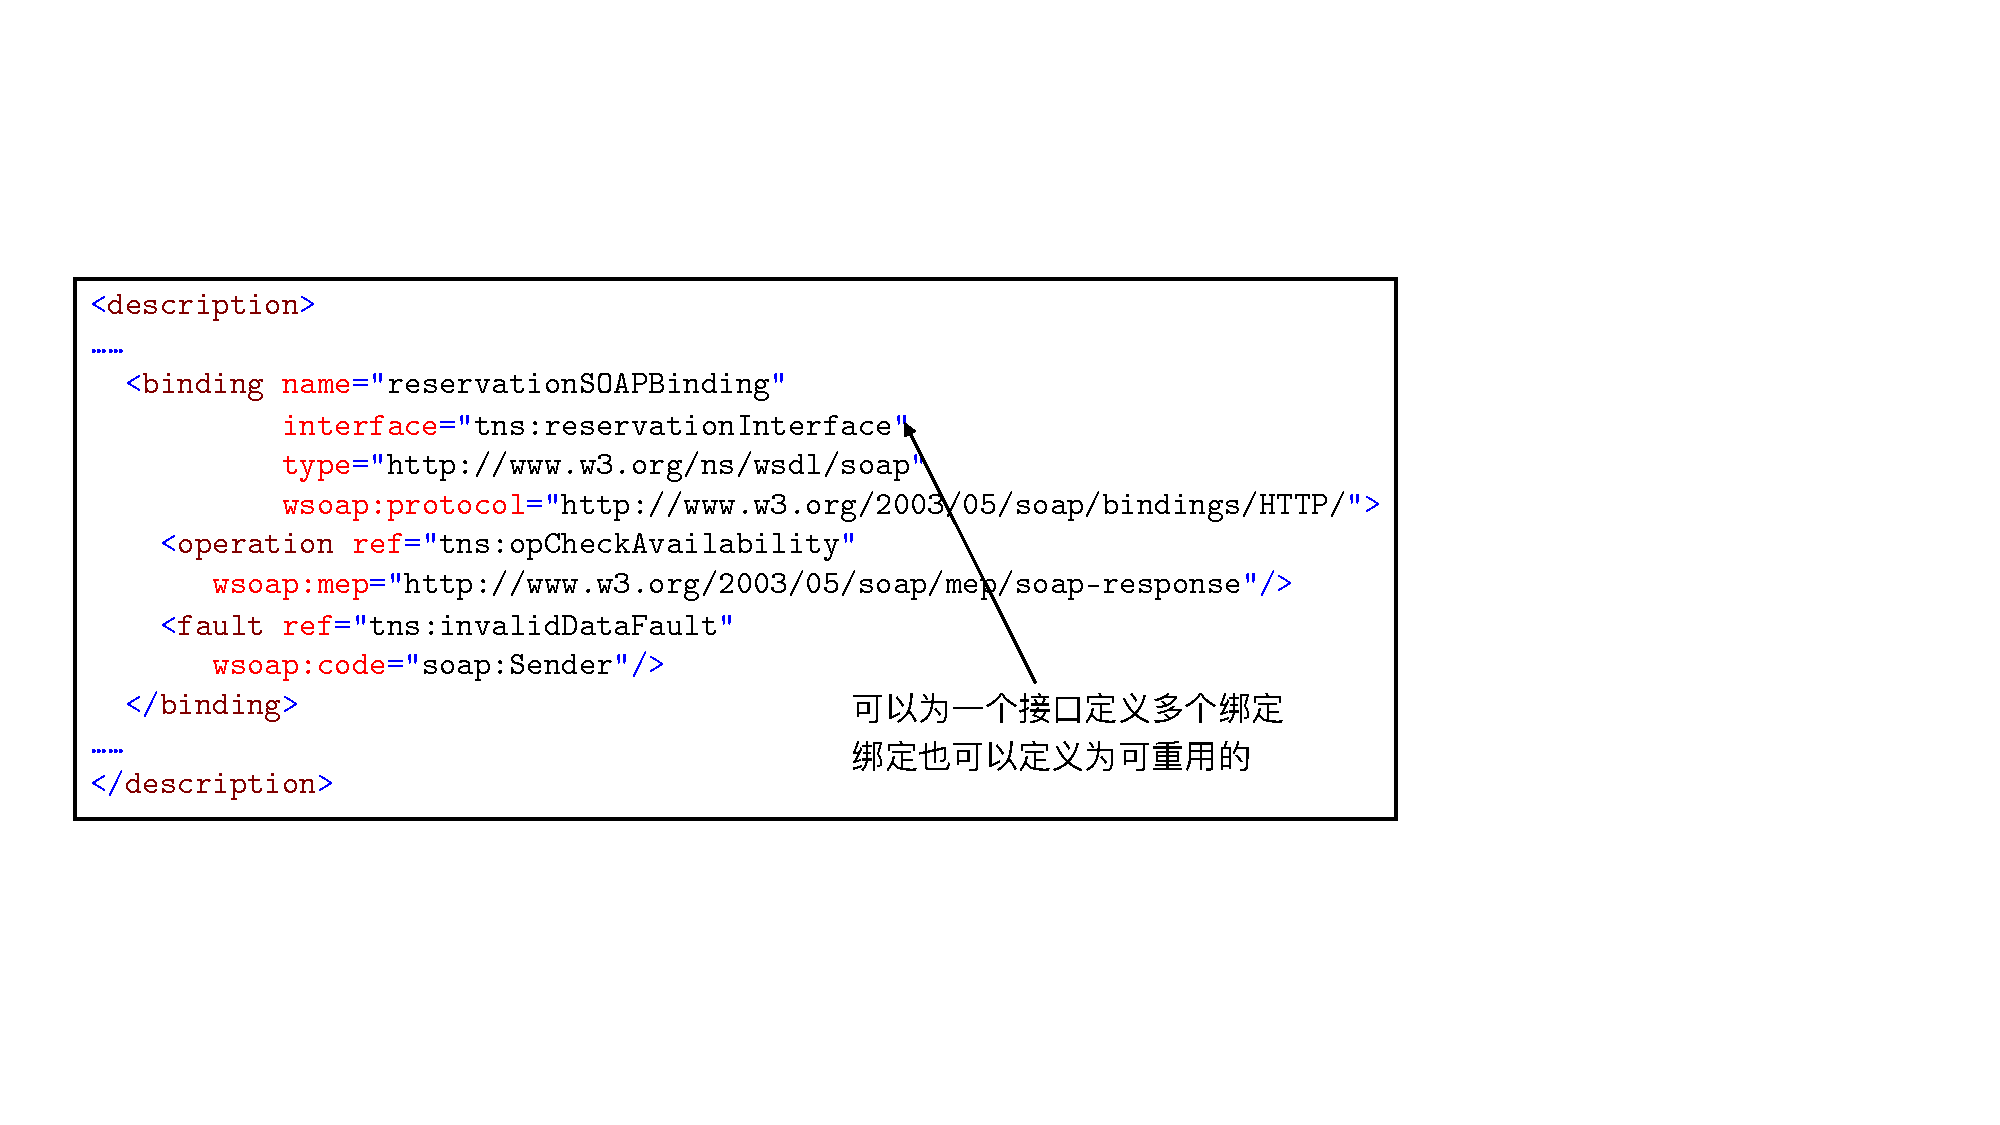
\includegraphics[width=0.87\textwidth]{images/定义绑定binding.pdf}
    \vspace{-1.5em}
\end{figure}

\paragraph*{定义服务service}~{} \par
\begin{figure}[H]
    \vspace{-0.7em}
	\centering
	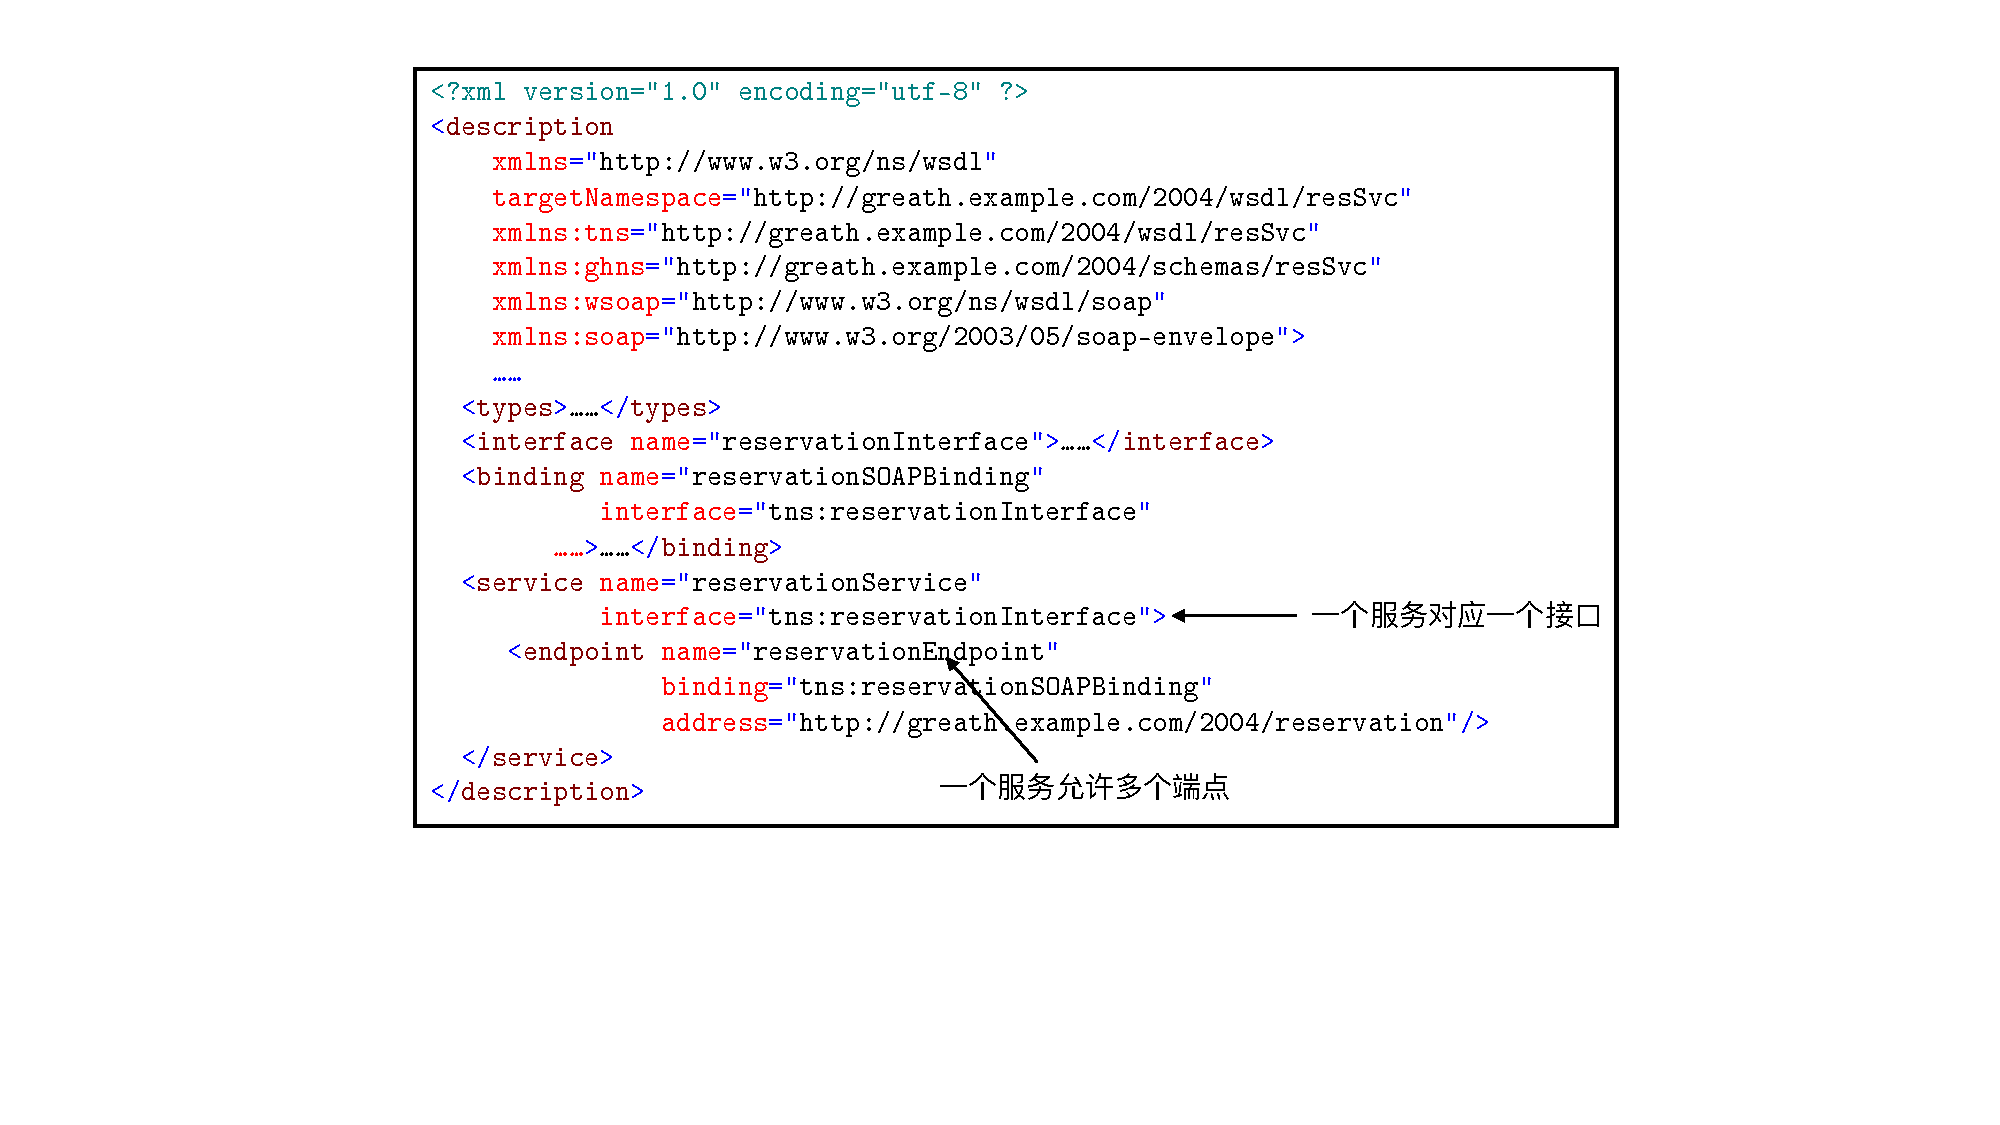
\includegraphics[width=0.93\textwidth]{images/定义服务service.pdf}
    \vspace{-1.5em}
\end{figure}

\paragraph*{文档化服务}~{} \par
\begin{figure}[H]
    \vspace{-0.7em}
	\centering
	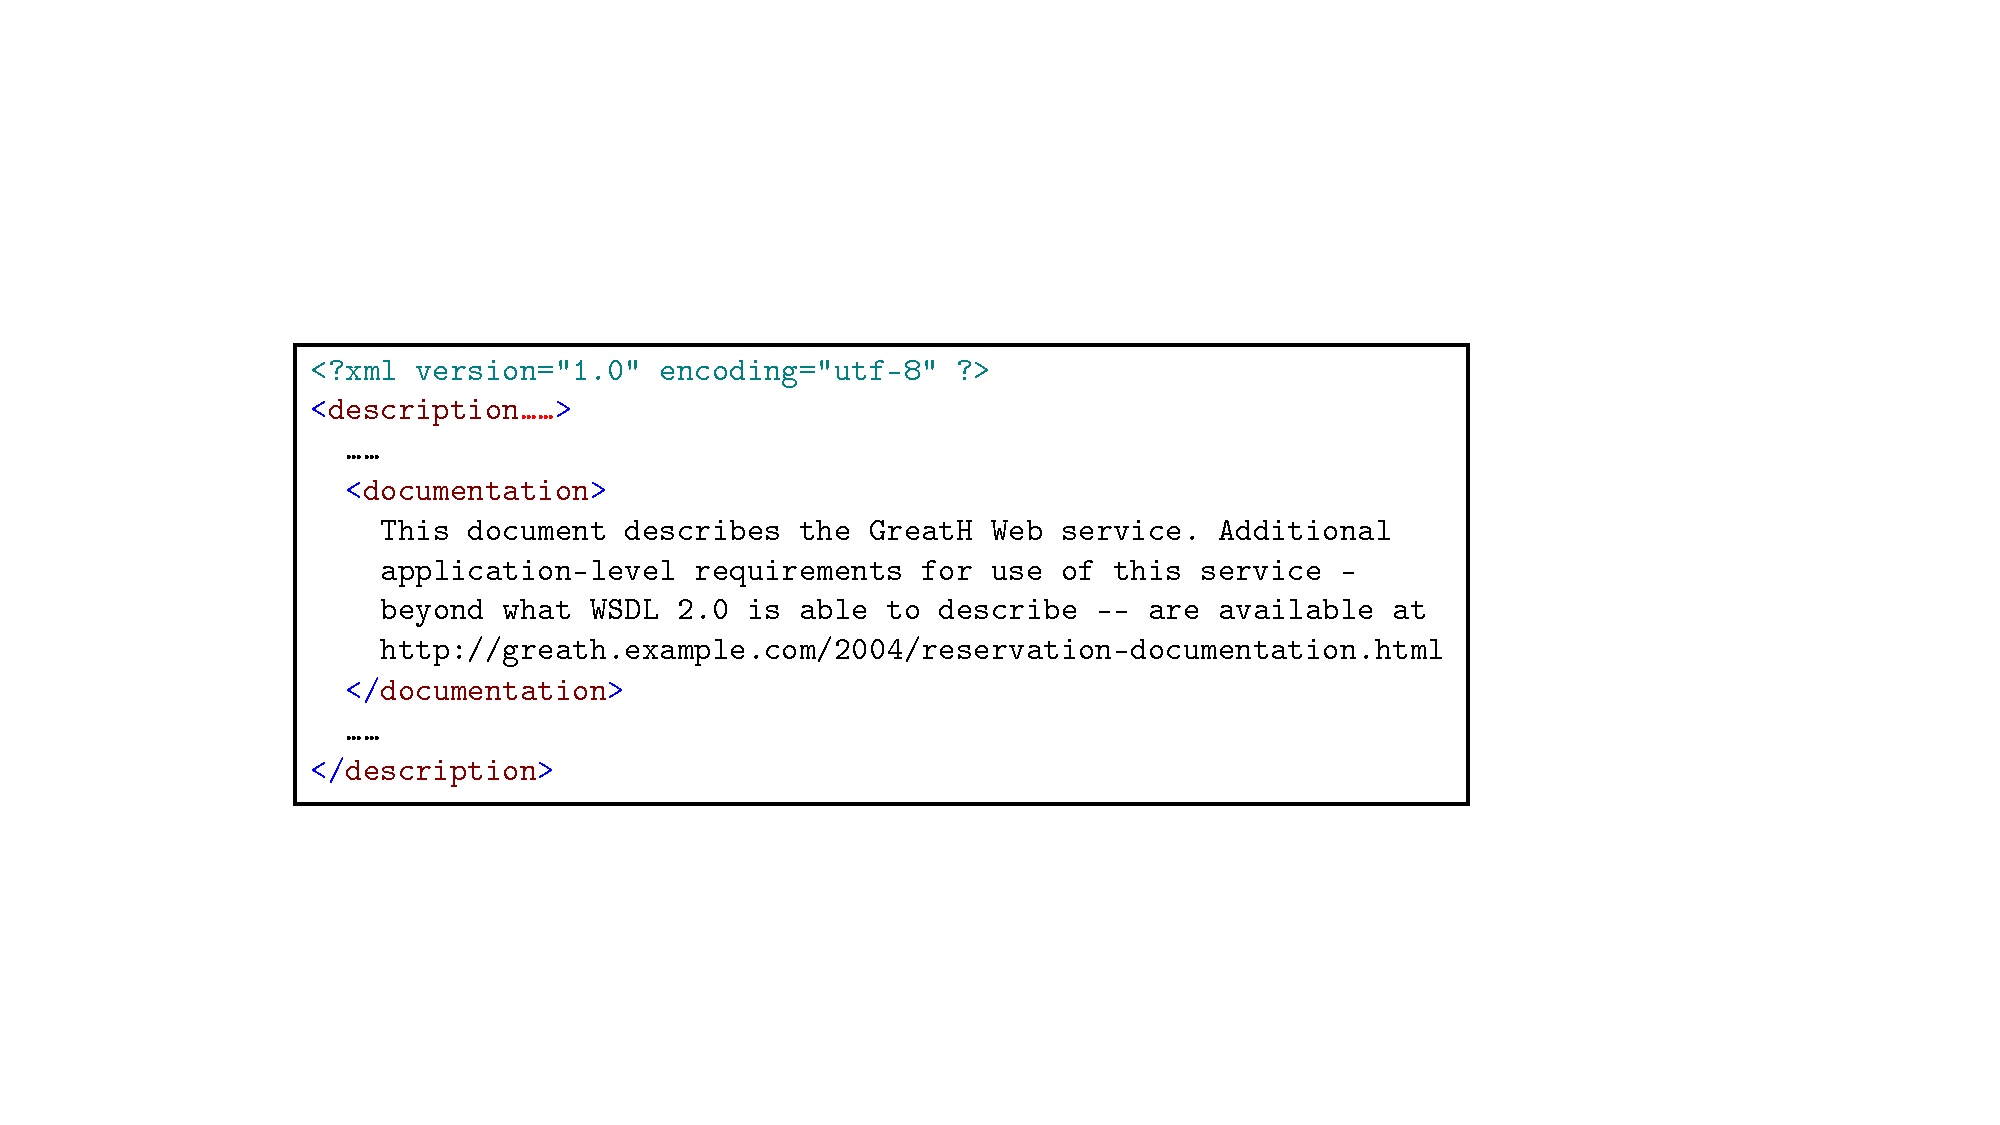
\includegraphics[width=0.83\textwidth]{images/文档化服务.pdf}
    \vspace{-1.5em}
\end{figure}

\paragraph*{RPC风格}~{} \par
\begin{figure}[H]
    \vspace{-0.7em}
	\centering
	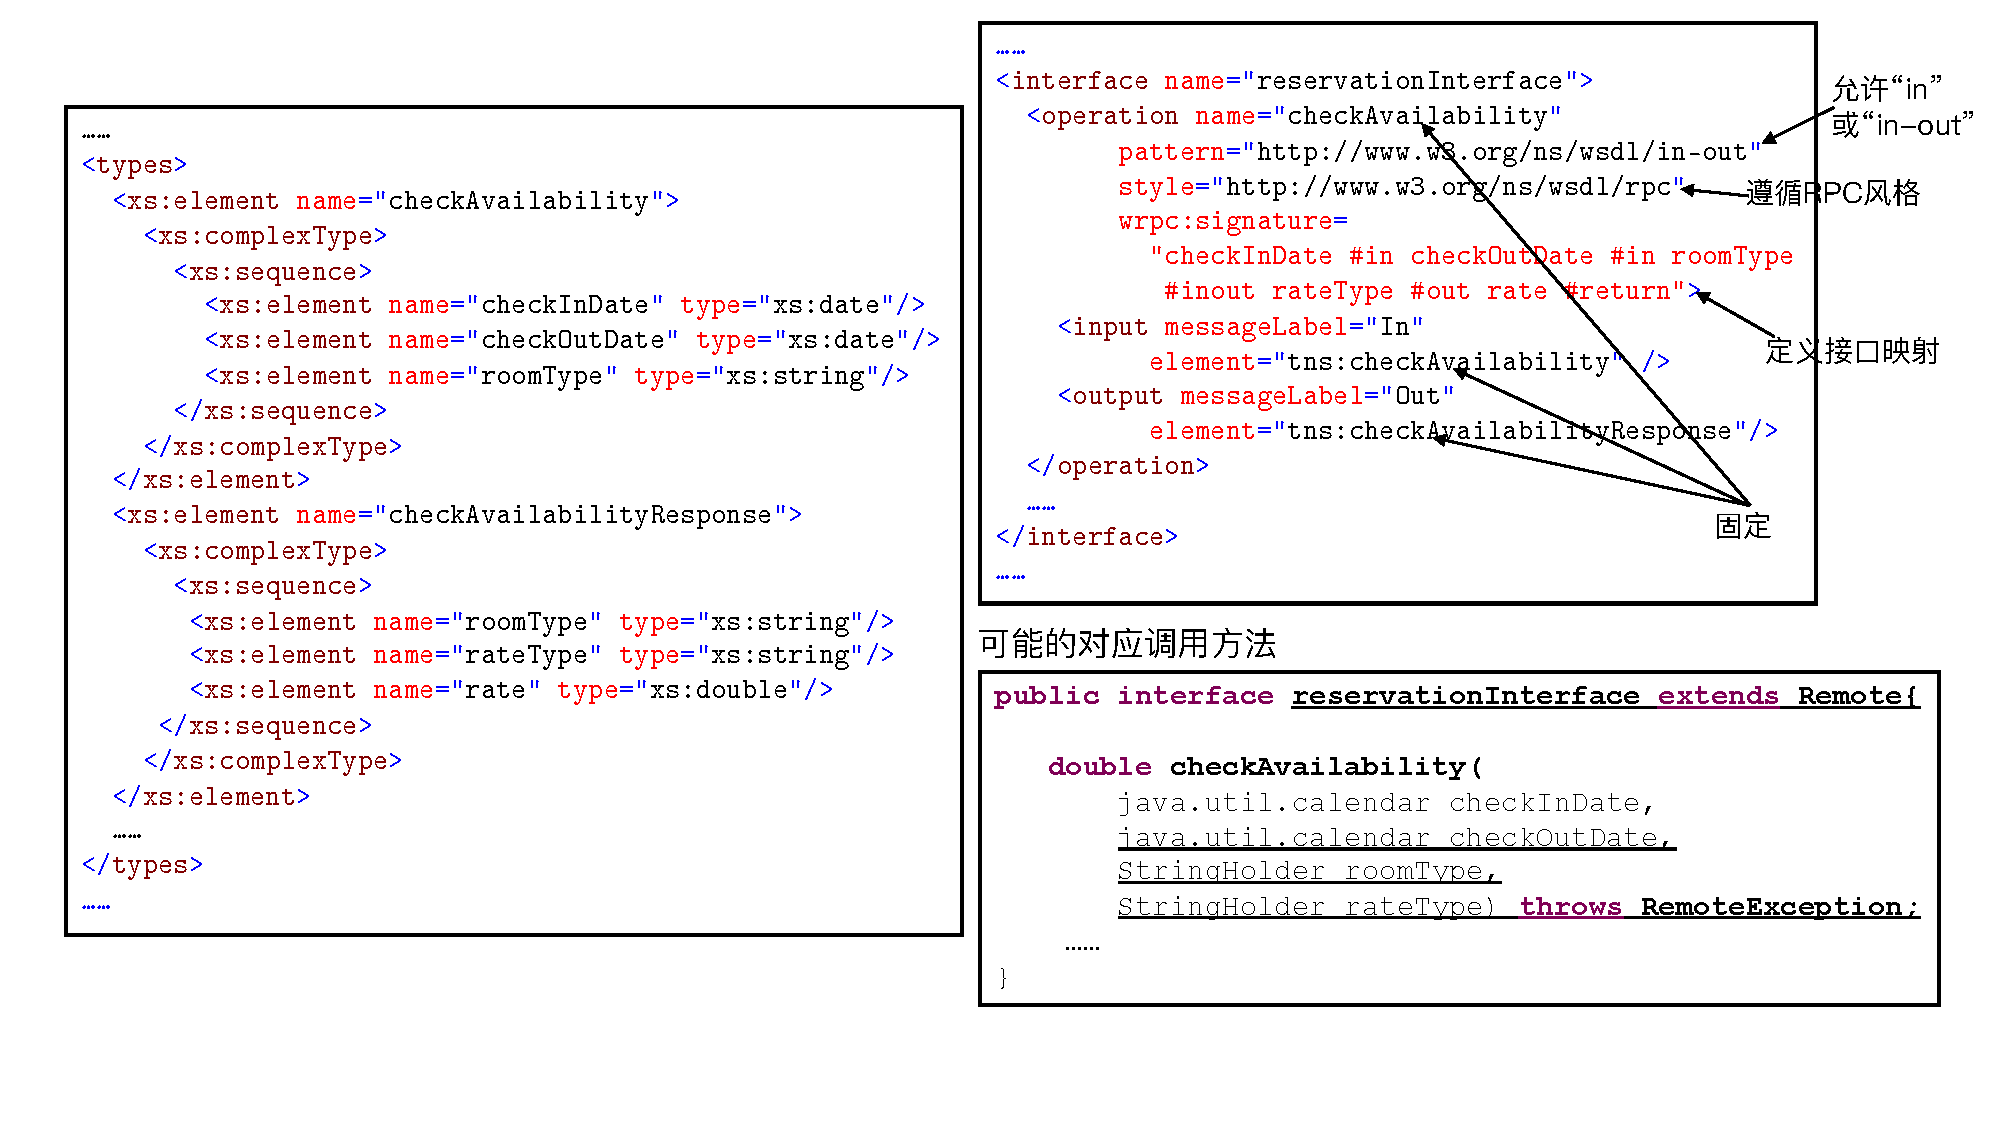
\includegraphics[width=\textwidth]{images/RPC风格.pdf}
    \vspace{-1.5em}
\end{figure}

\subsubsection{WSDL简化结构}
\begin{figure}[H]
    \vspace{-0.7em}
	\centering
	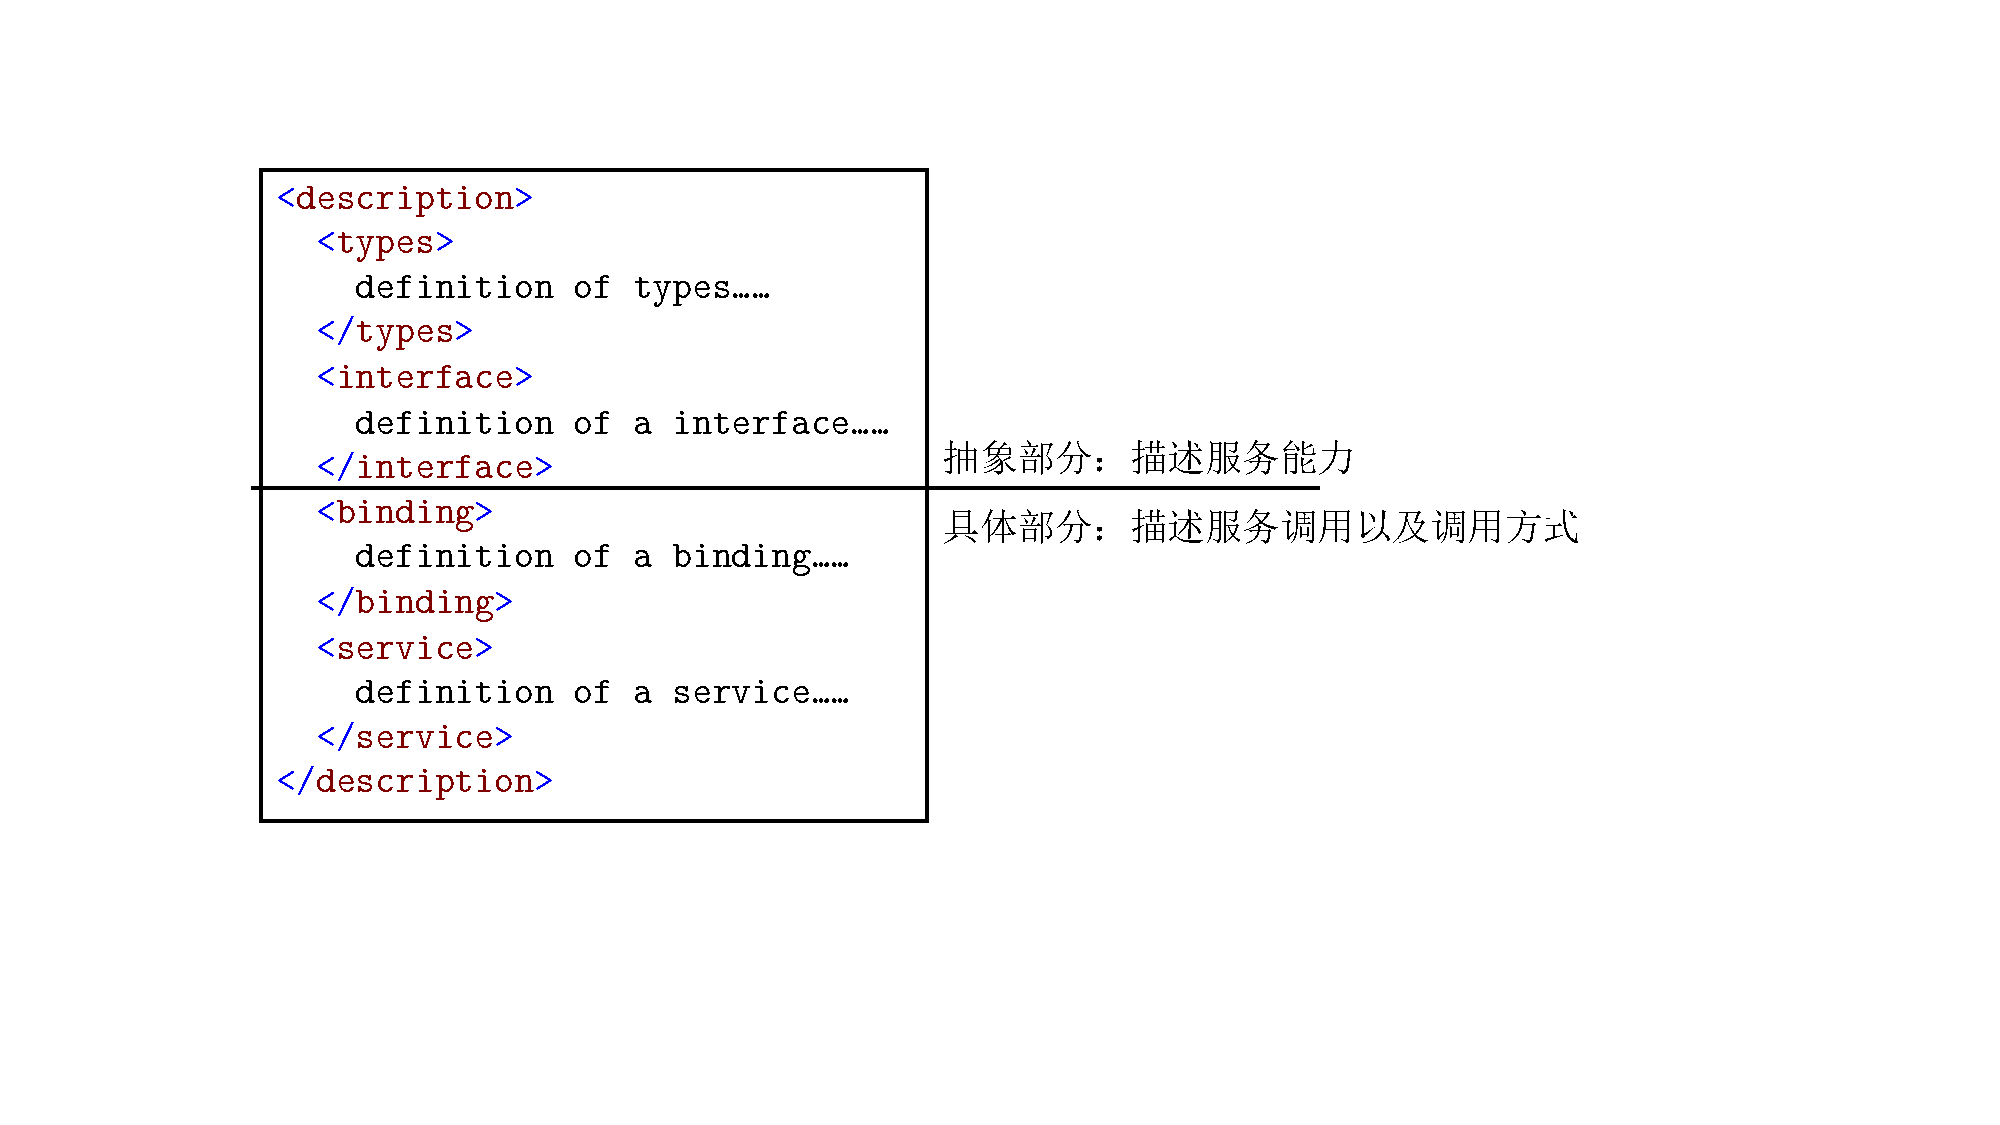
\includegraphics[width=0.75\textwidth]{images/WSDL简化结构.pdf}
    \vspace{-1em}
\end{figure}

\begin{figure}[H]
    \vspace{-0.7em}
	\centering
	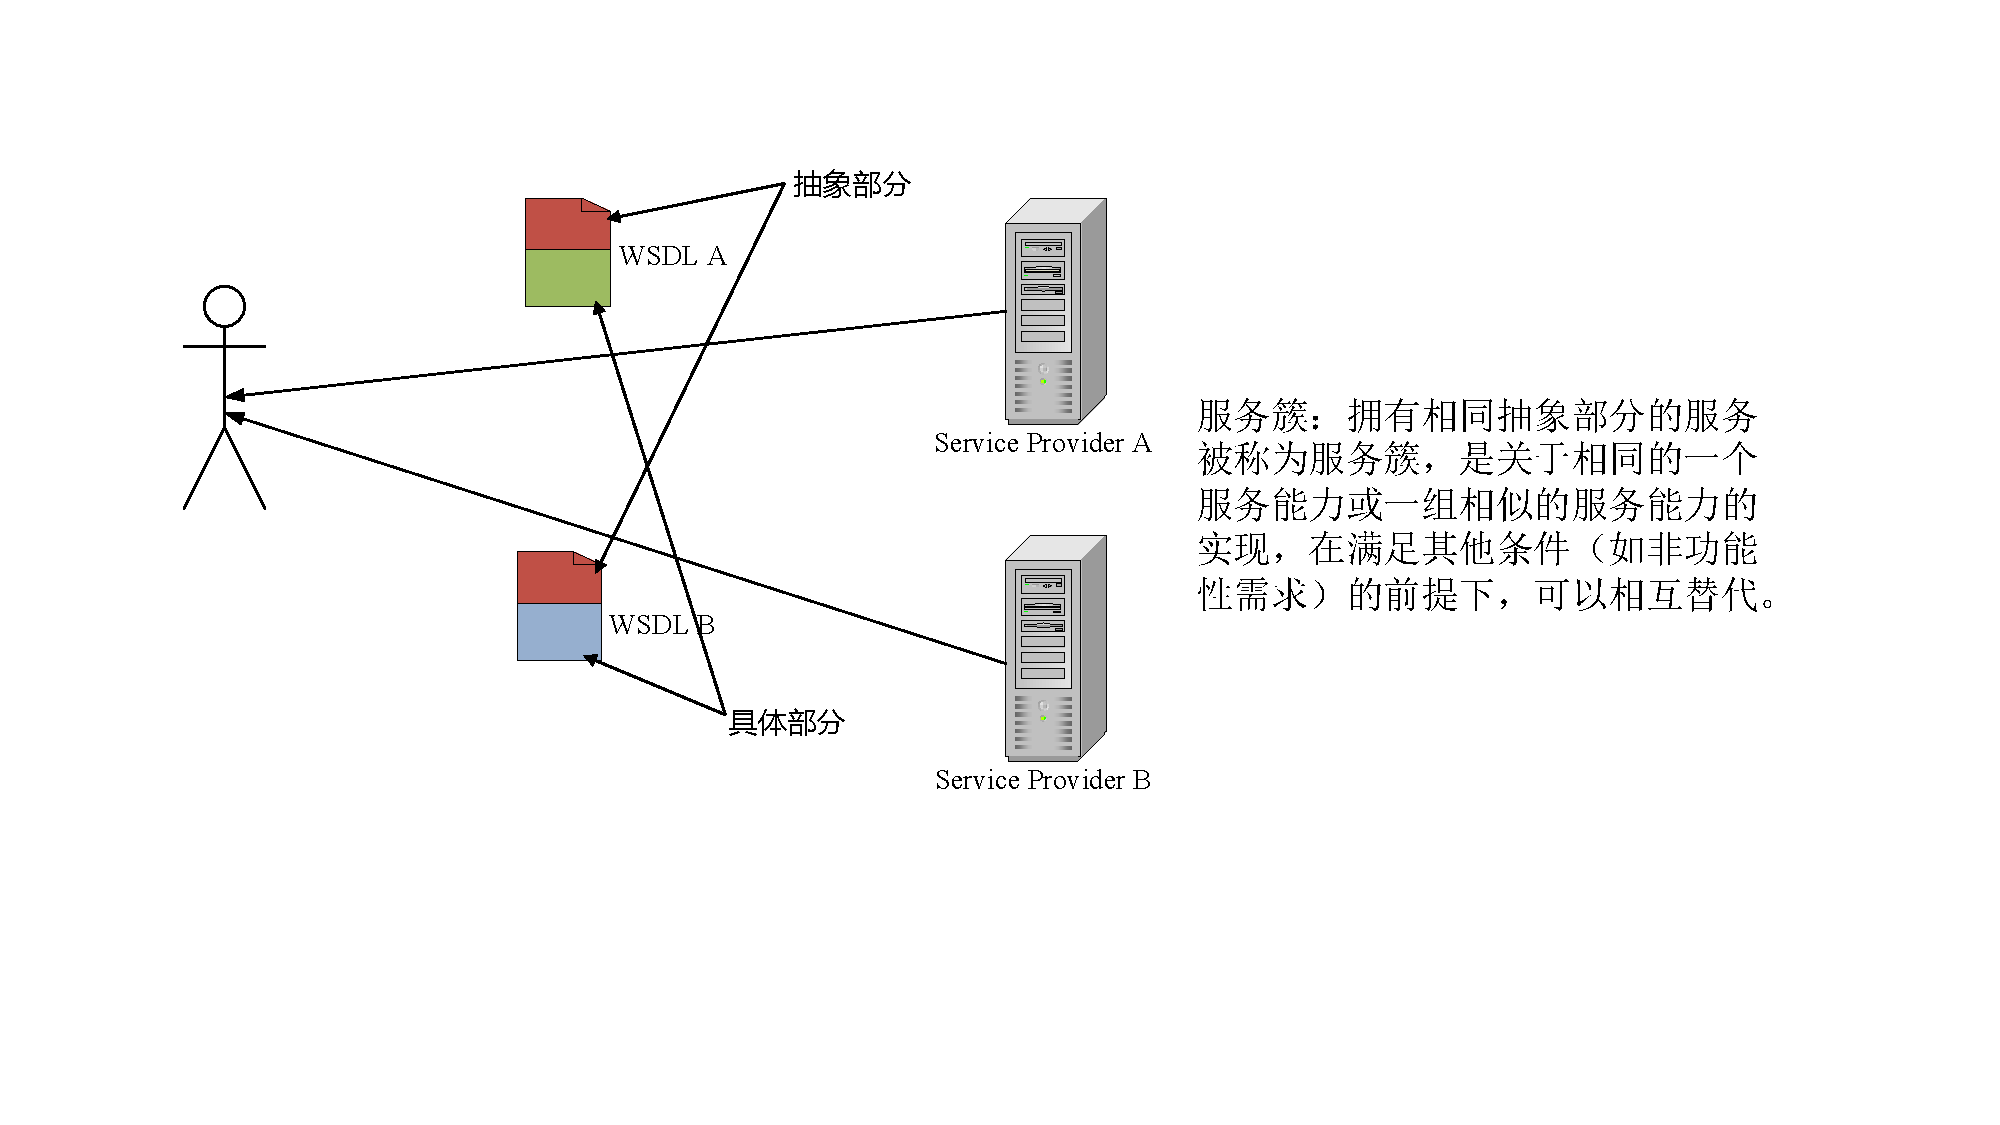
\includegraphics[width=0.9\textwidth]{images/服务簇.pdf}
    \vspace{-1em}
\end{figure}

\subsubsection{WSDL 1.1与WSDL 2.0的差异}
一方面是一些名称上的差异(portType和interface、port和endpoint);另一方面在WSDL 1.1中有一个单独用来说明中继消息message的element,而WSDL 2.0中没有。
\begin{figure}[H]
    \vspace{-0.7em}
	\centering
	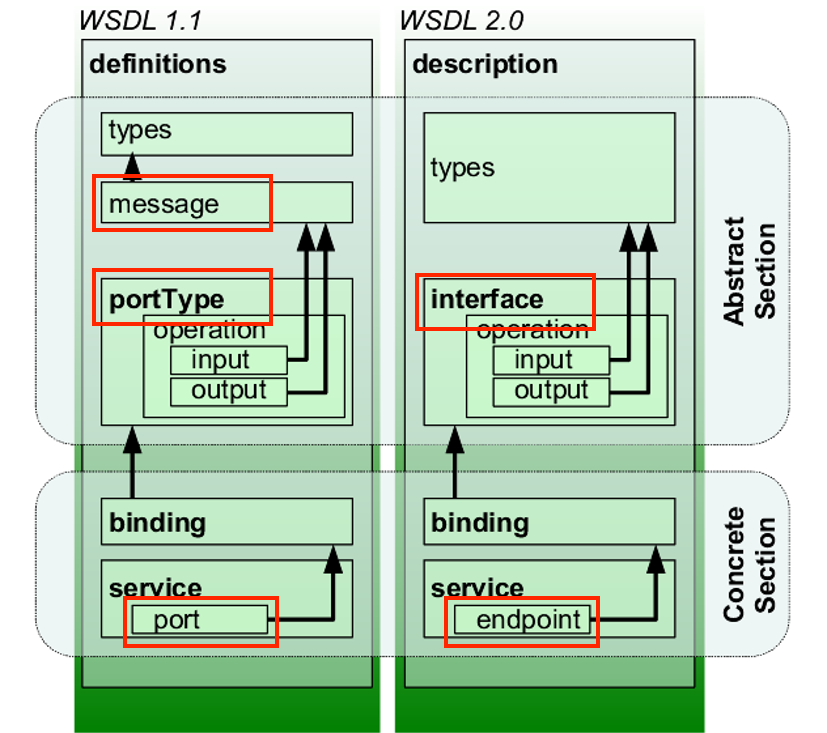
\includegraphics[width=0.55\textwidth]{images/WSDL 1.1与WSDL 2.0的差异.png}
    \vspace{-1em}
\end{figure}

\subsection{BPEL}

\subsubsection{BPEL的引入}
\begin{itemize}
    \item 现在我们有:
    \vspace{-0.8em}
    \begin{multicols}{2}
        \begin{itemize}
            \item XML,Namespace,XML Schema,SOAP
            \item WSDL用来定义服务/服务能力
        \end{itemize}
    \end{multicols}
    \vspace{-1em}
    \item 下一个问题是:为了建模服务,XML,SOAP,WSDL是不是足够了?
    \begin{itemize}
        \item 一个可能的答案,是的
        \item 另一个可能,对于更加复杂的服务,仍然不够
        \vspace{-1.2em}
        \begin{multicols}{2}
            \begin{itemize}
                \item 一个复合服务(WS-BPEL,WS-CDL)
                \item 一个带非功能性需求的服务(WS-*)
                \item 服务提供方和服务调用方之间交换信息的其他方法
            \end{itemize}
        \end{multicols}
        \vspace{-1em}
    \end{itemize}
\end{itemize}

\subsubsection{复合服务}
为什么需要复合服务:复用和灵活
\begin{itemize}
    \item 有些服务是垂直的,有些服务是水平的。为保证复用性,某些垂直服务被设计为由水平服务构造而来
    \item 如果活动由服务实现,那么由活动构成的(商业)流程由复合服务实现
\end{itemize}

如何实现复合服务:
\begin{itemize}
    \item 一个可能的方法,在传统编程环境中,调用子服务,再把编程单元封装成服务以供调用
    \item 采用标准协议的XML脚本描述服务组合方式
\end{itemize}

建模复合Web服务:要建模一个涉及多个参与方的业务流程,可能需要多个Web服务协作来形成一个复合Web服务,它们在逻辑上是独立的,可能由不同的提供者实现。

\subsubsection{BPEL的概念}
业务流程执行语言(Business Process Execution Language, BPEL4WS、WS4BPEL、BPEL或WS-BPEL)是一种用于协调Web服务以实现全面业务流程的流程表示方式。BPEL是一种基于XML的,用来描写业务过程的编程语言,被描写的业务过程的每个单一步骤则由Web服务来实现。
\begin{itemize}
    \item 定义了一种互操作的集成模型,以促进自动化流程集成在企业内部和企业之间环境中的扩展。
    \item BPEL流程定义了如何协调多个业务交互以实现共同的业务目标,并具有必要的状态和逻辑来进行协调。
    \item 精确定义了跨企业业务协议的基本服务行为,例如:
    \vspace{-0.8em}
    \begin{multicols}{3}
        \begin{itemize}
            \item 数据相关行为
            \item 异常情况及其后果
            \item 各粒度的长时间运行交互
        \end{itemize}
    \end{multicols}
    \vspace{-1em}
    \item 将业务流程的公共行为与其内部实现分离开来。
    \item 有两种方式可以对业务流程进行建模:
    \begin{itemize}
        \item 可执行的流程模型:模拟业务交互参与方的实际行为
        \item 抽象模型:指定涉及方的互相可见的消息交换行为,而不揭示它们的内部行为
    \end{itemize}
    \item 在BPEL中创建业务流程的两个步骤:
    \vspace{-0.8em}
    \begin{multicols}{2}
        \begin{itemize}
            \item 创建服务描述
            \item 创建业务流程
        \end{itemize}
    \end{multicols}
    \vspace{-1em}
\end{itemize}

\subsubsection{一个简单的复合Web Service}
\begin{figure}[H]
    \vspace{-0.7em}
	\centering
	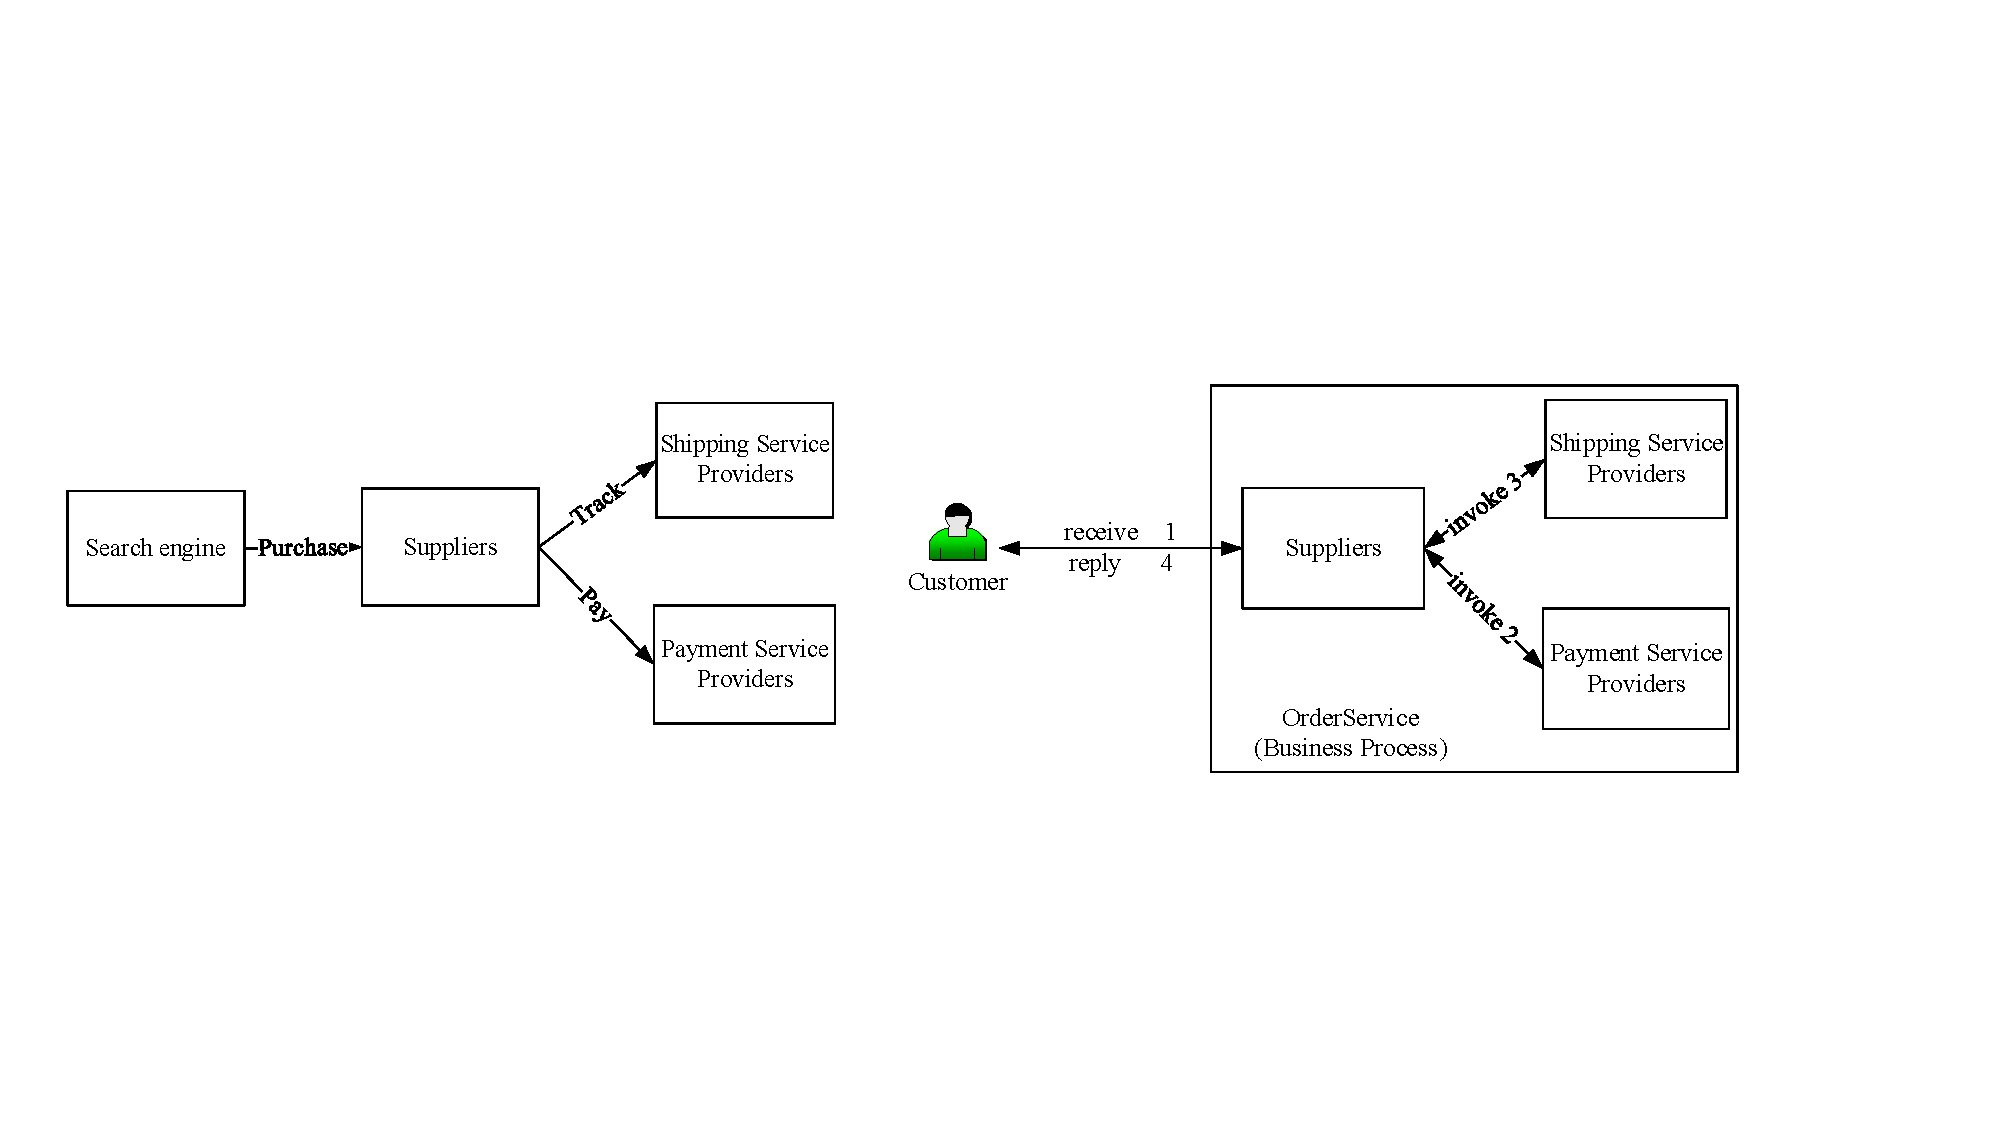
\includegraphics[width=0.92\textwidth]{images/一个简单的复合Web Service.pdf}
    \vspace{-1.5em}
\end{figure}

\subsubsection{BPEL应用实例}
\paragraph*{创建服务描述}~{} \par
使用 WSDL 定义相关方和消息(用于支付和运输提供商Shipping/Payment Service Providers)
\begin{figure}[H]
    \vspace{-0.7em}
	\centering
	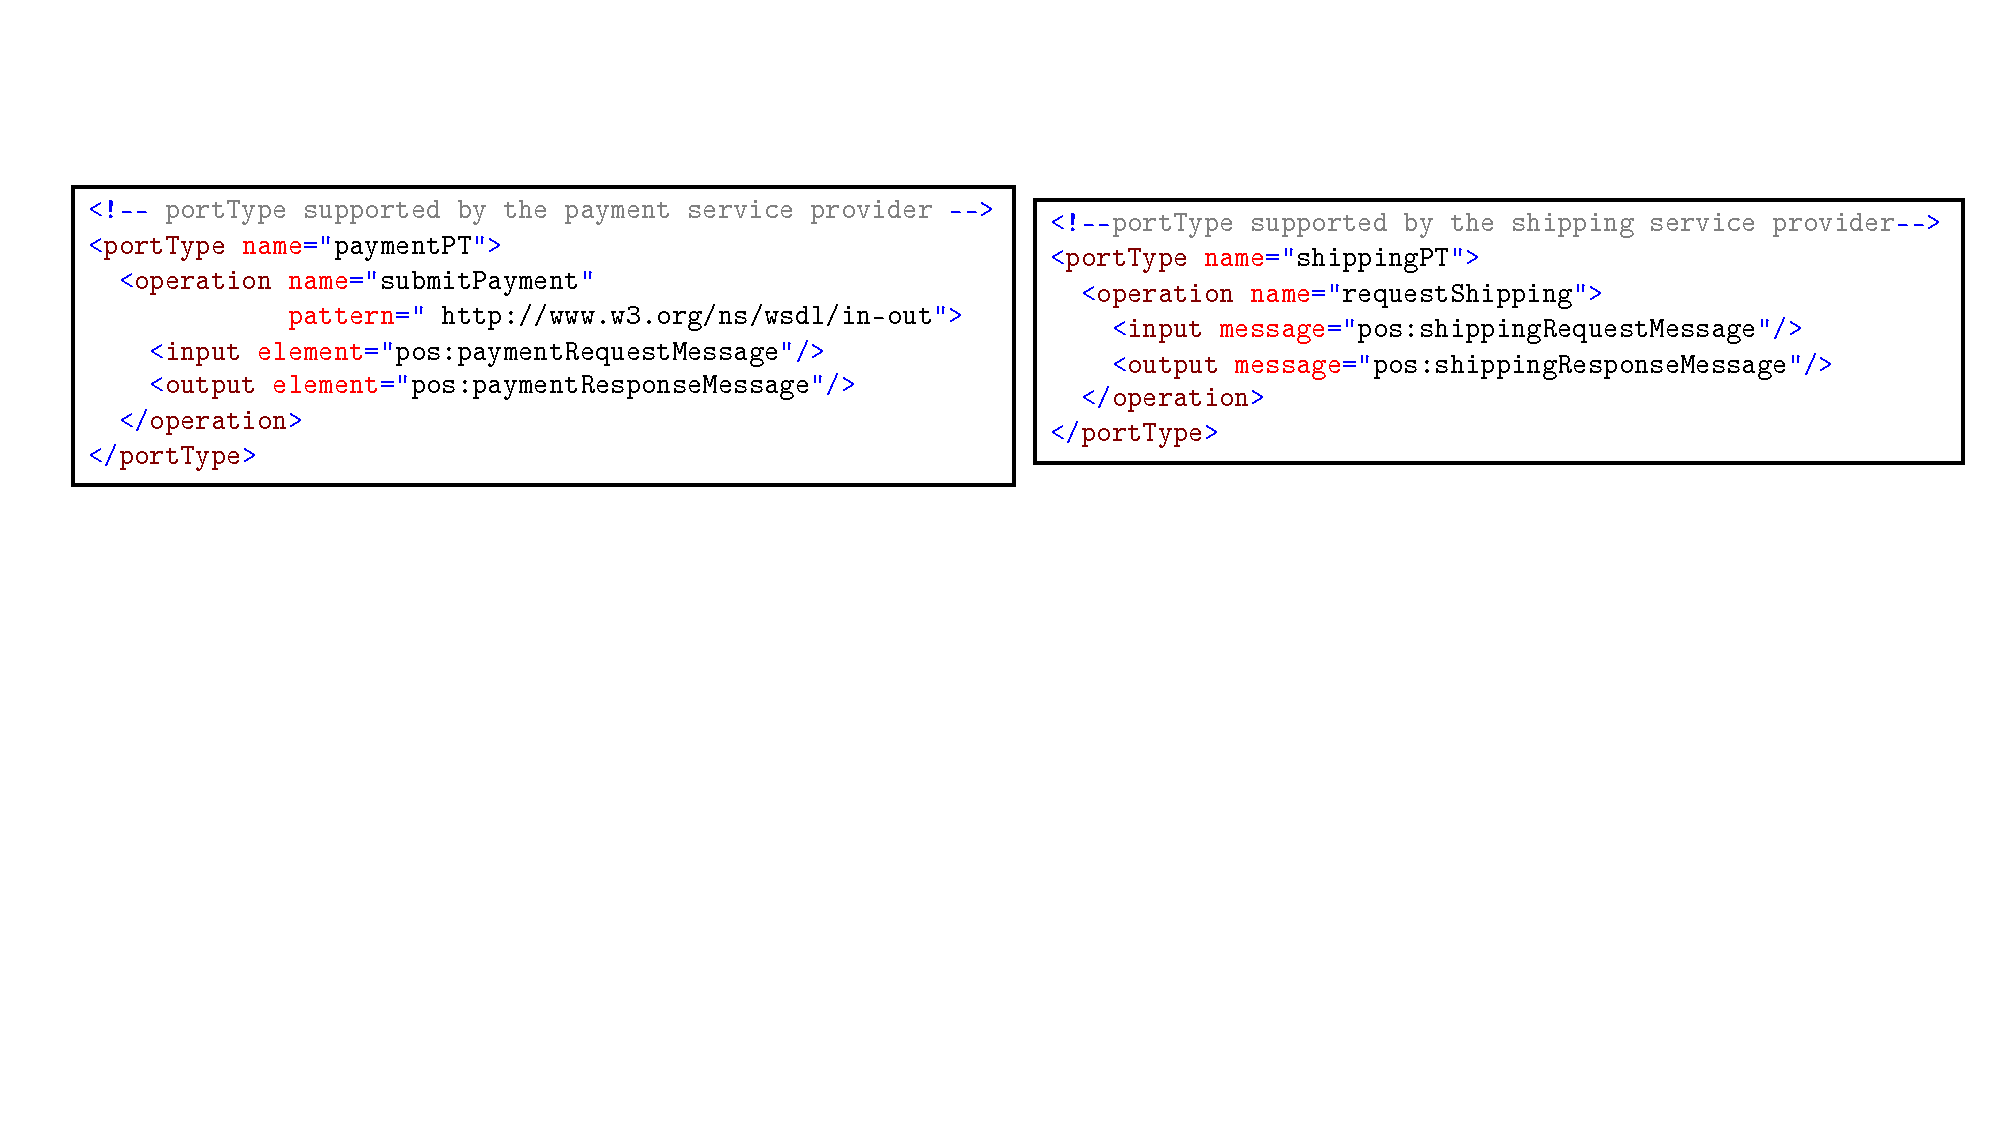
\includegraphics[width=0.95\textwidth]{images/创建服务描述.pdf}
    \vspace{-1.5em}
\end{figure}

使用WSDL定义供应商Suppliers
\begin{figure}[H]
    \vspace{-0.7em}
	\centering
	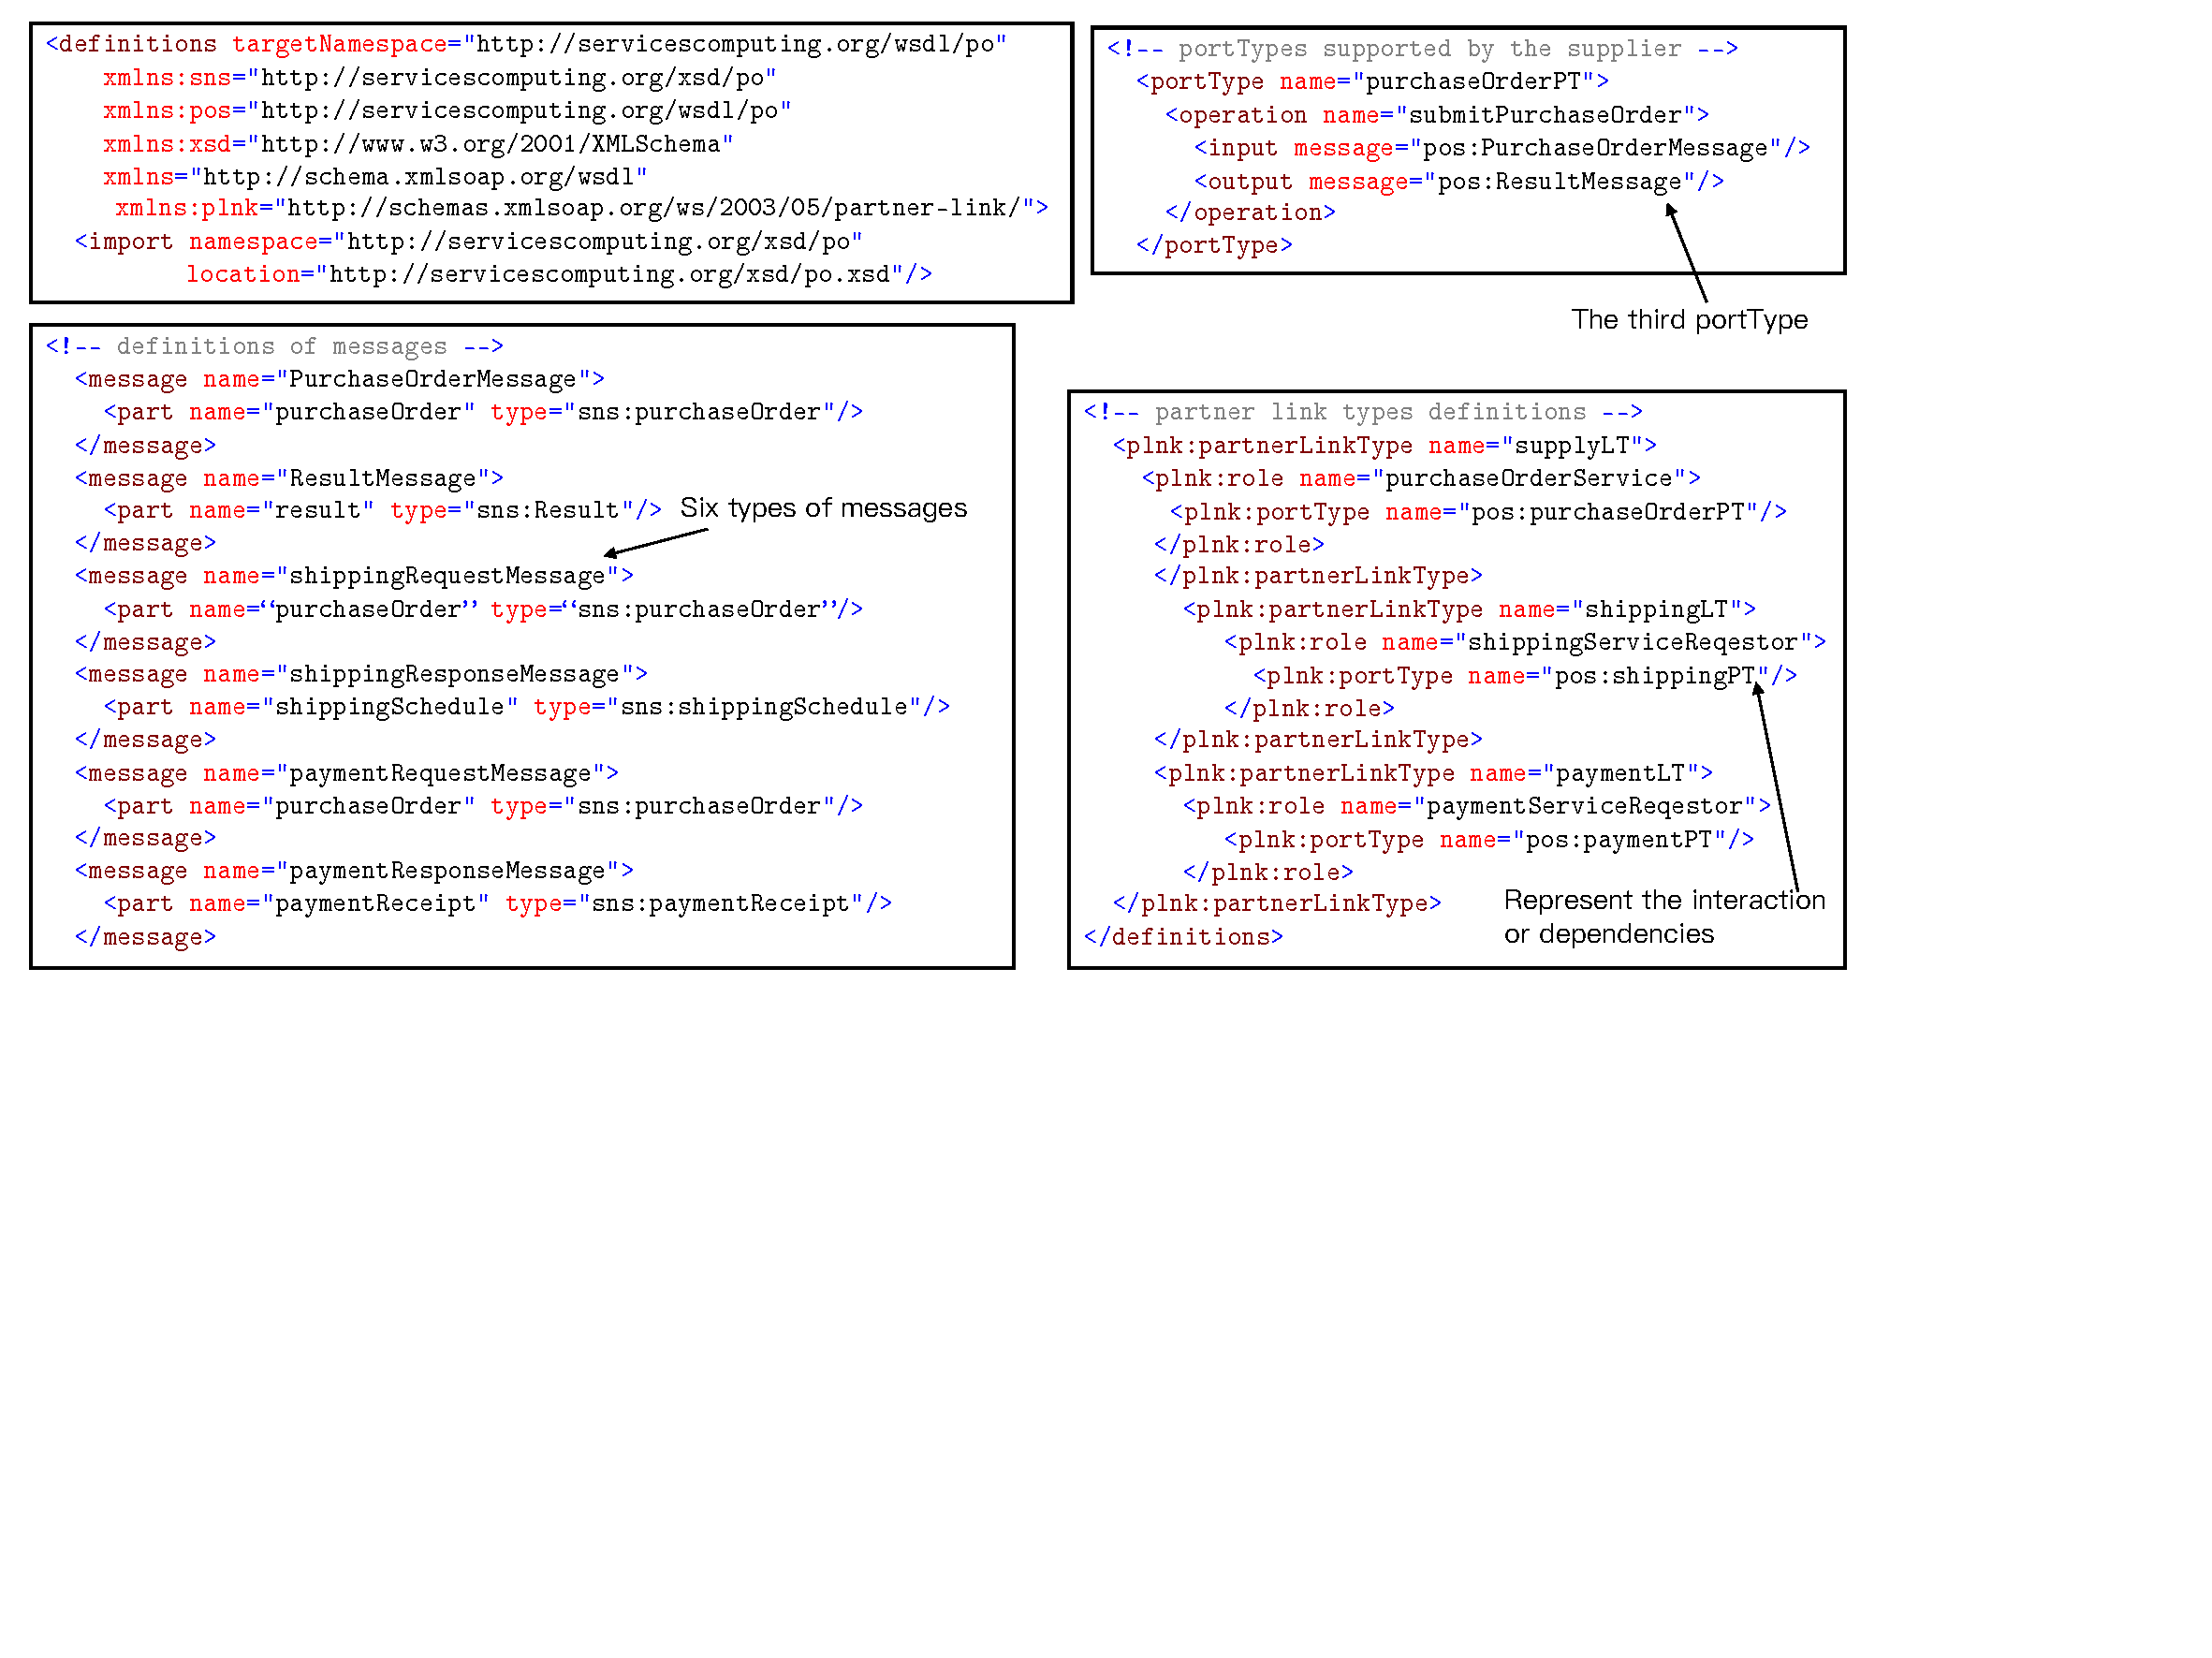
\includegraphics[width=\textwidth]{images/创建服务描述2.pdf}
    \vspace{-5.5em}
\end{figure}

\paragraph*{创建业务过程}~{} \par
可以使用端口类型、操作和消息类型的定义来详细说明流程
\begin{figure}[H]
    \vspace{-0.5em}
	\centering
	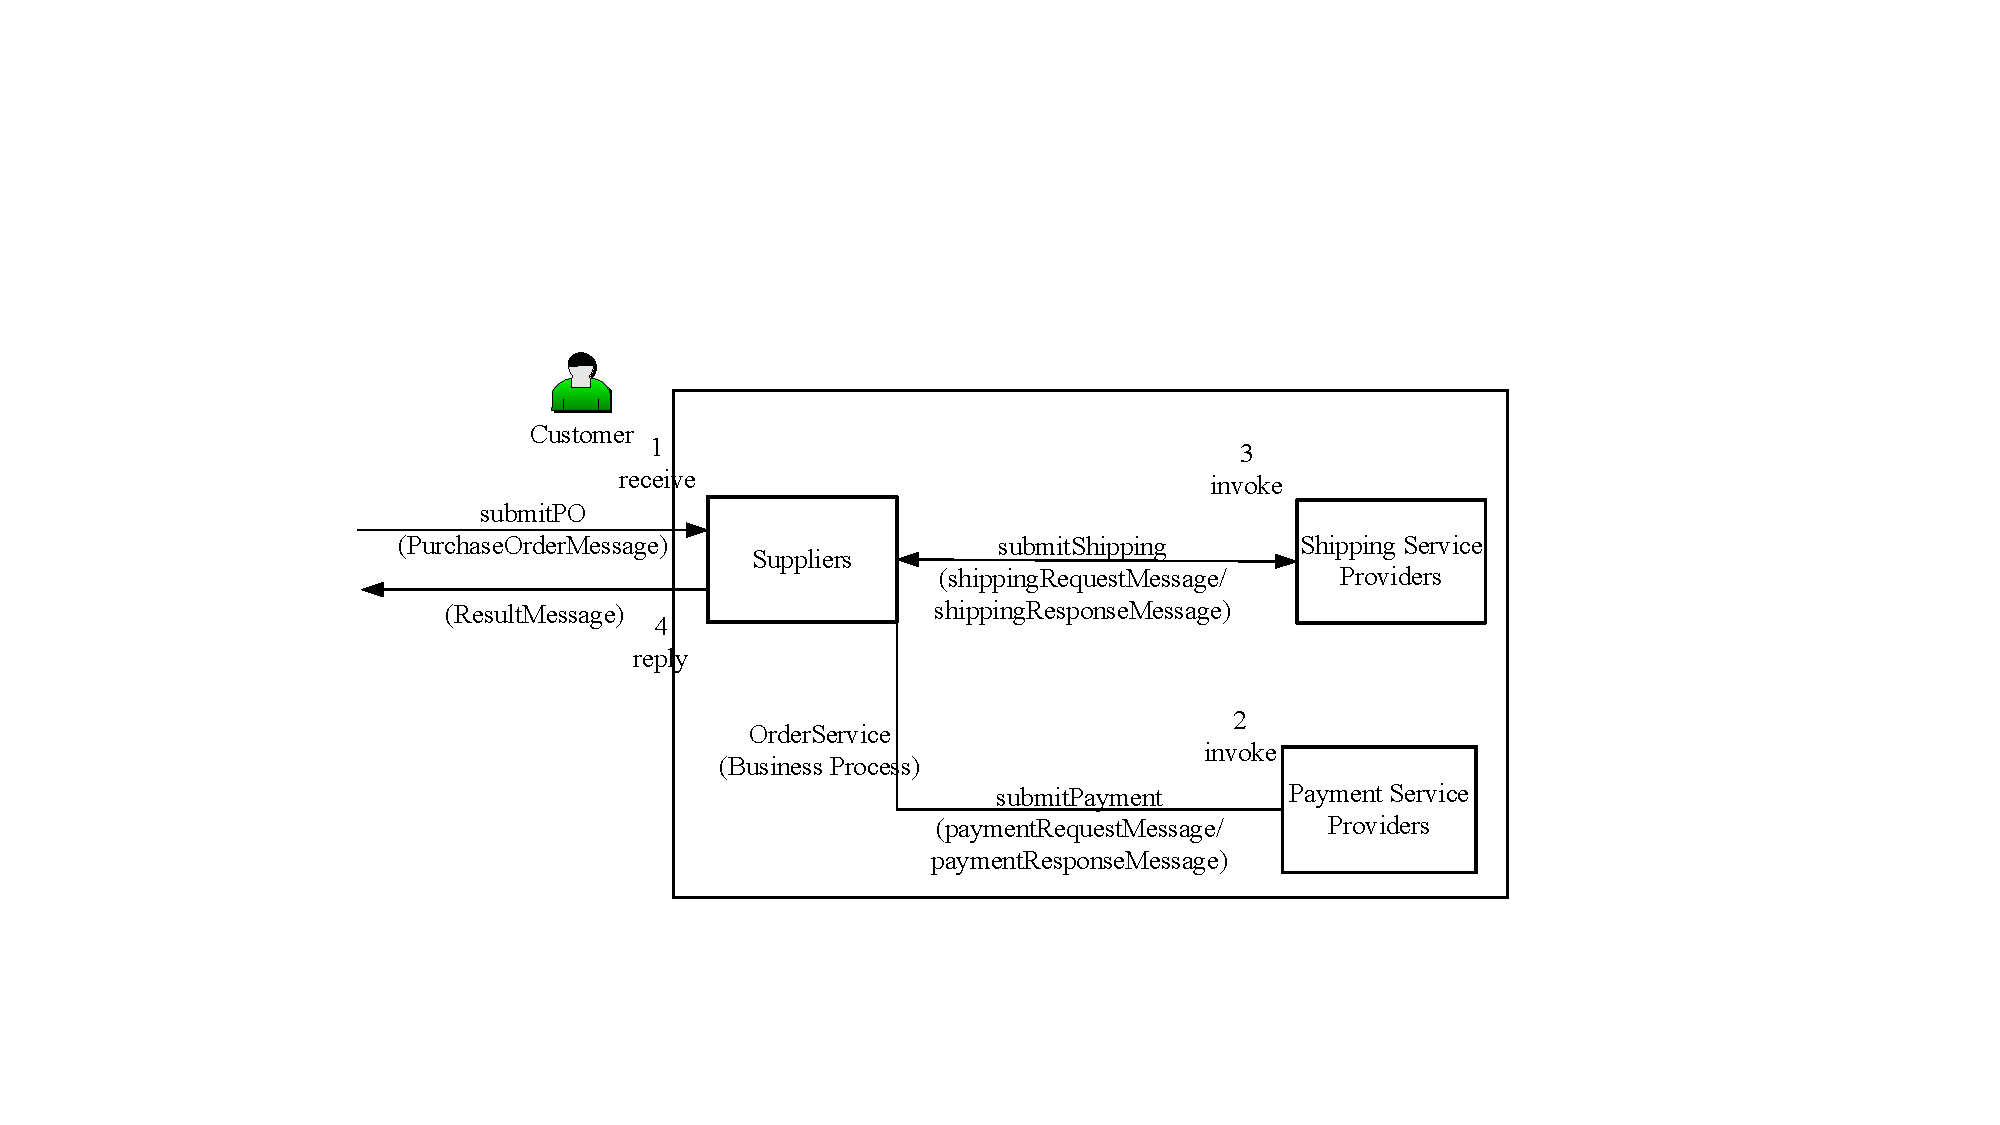
\includegraphics[width=0.7\textwidth]{images/创建业务过程.pdf}
    \vspace{-1em}
\end{figure}

\begin{figure}[H]
    \vspace{-0.5em}
	\centering
	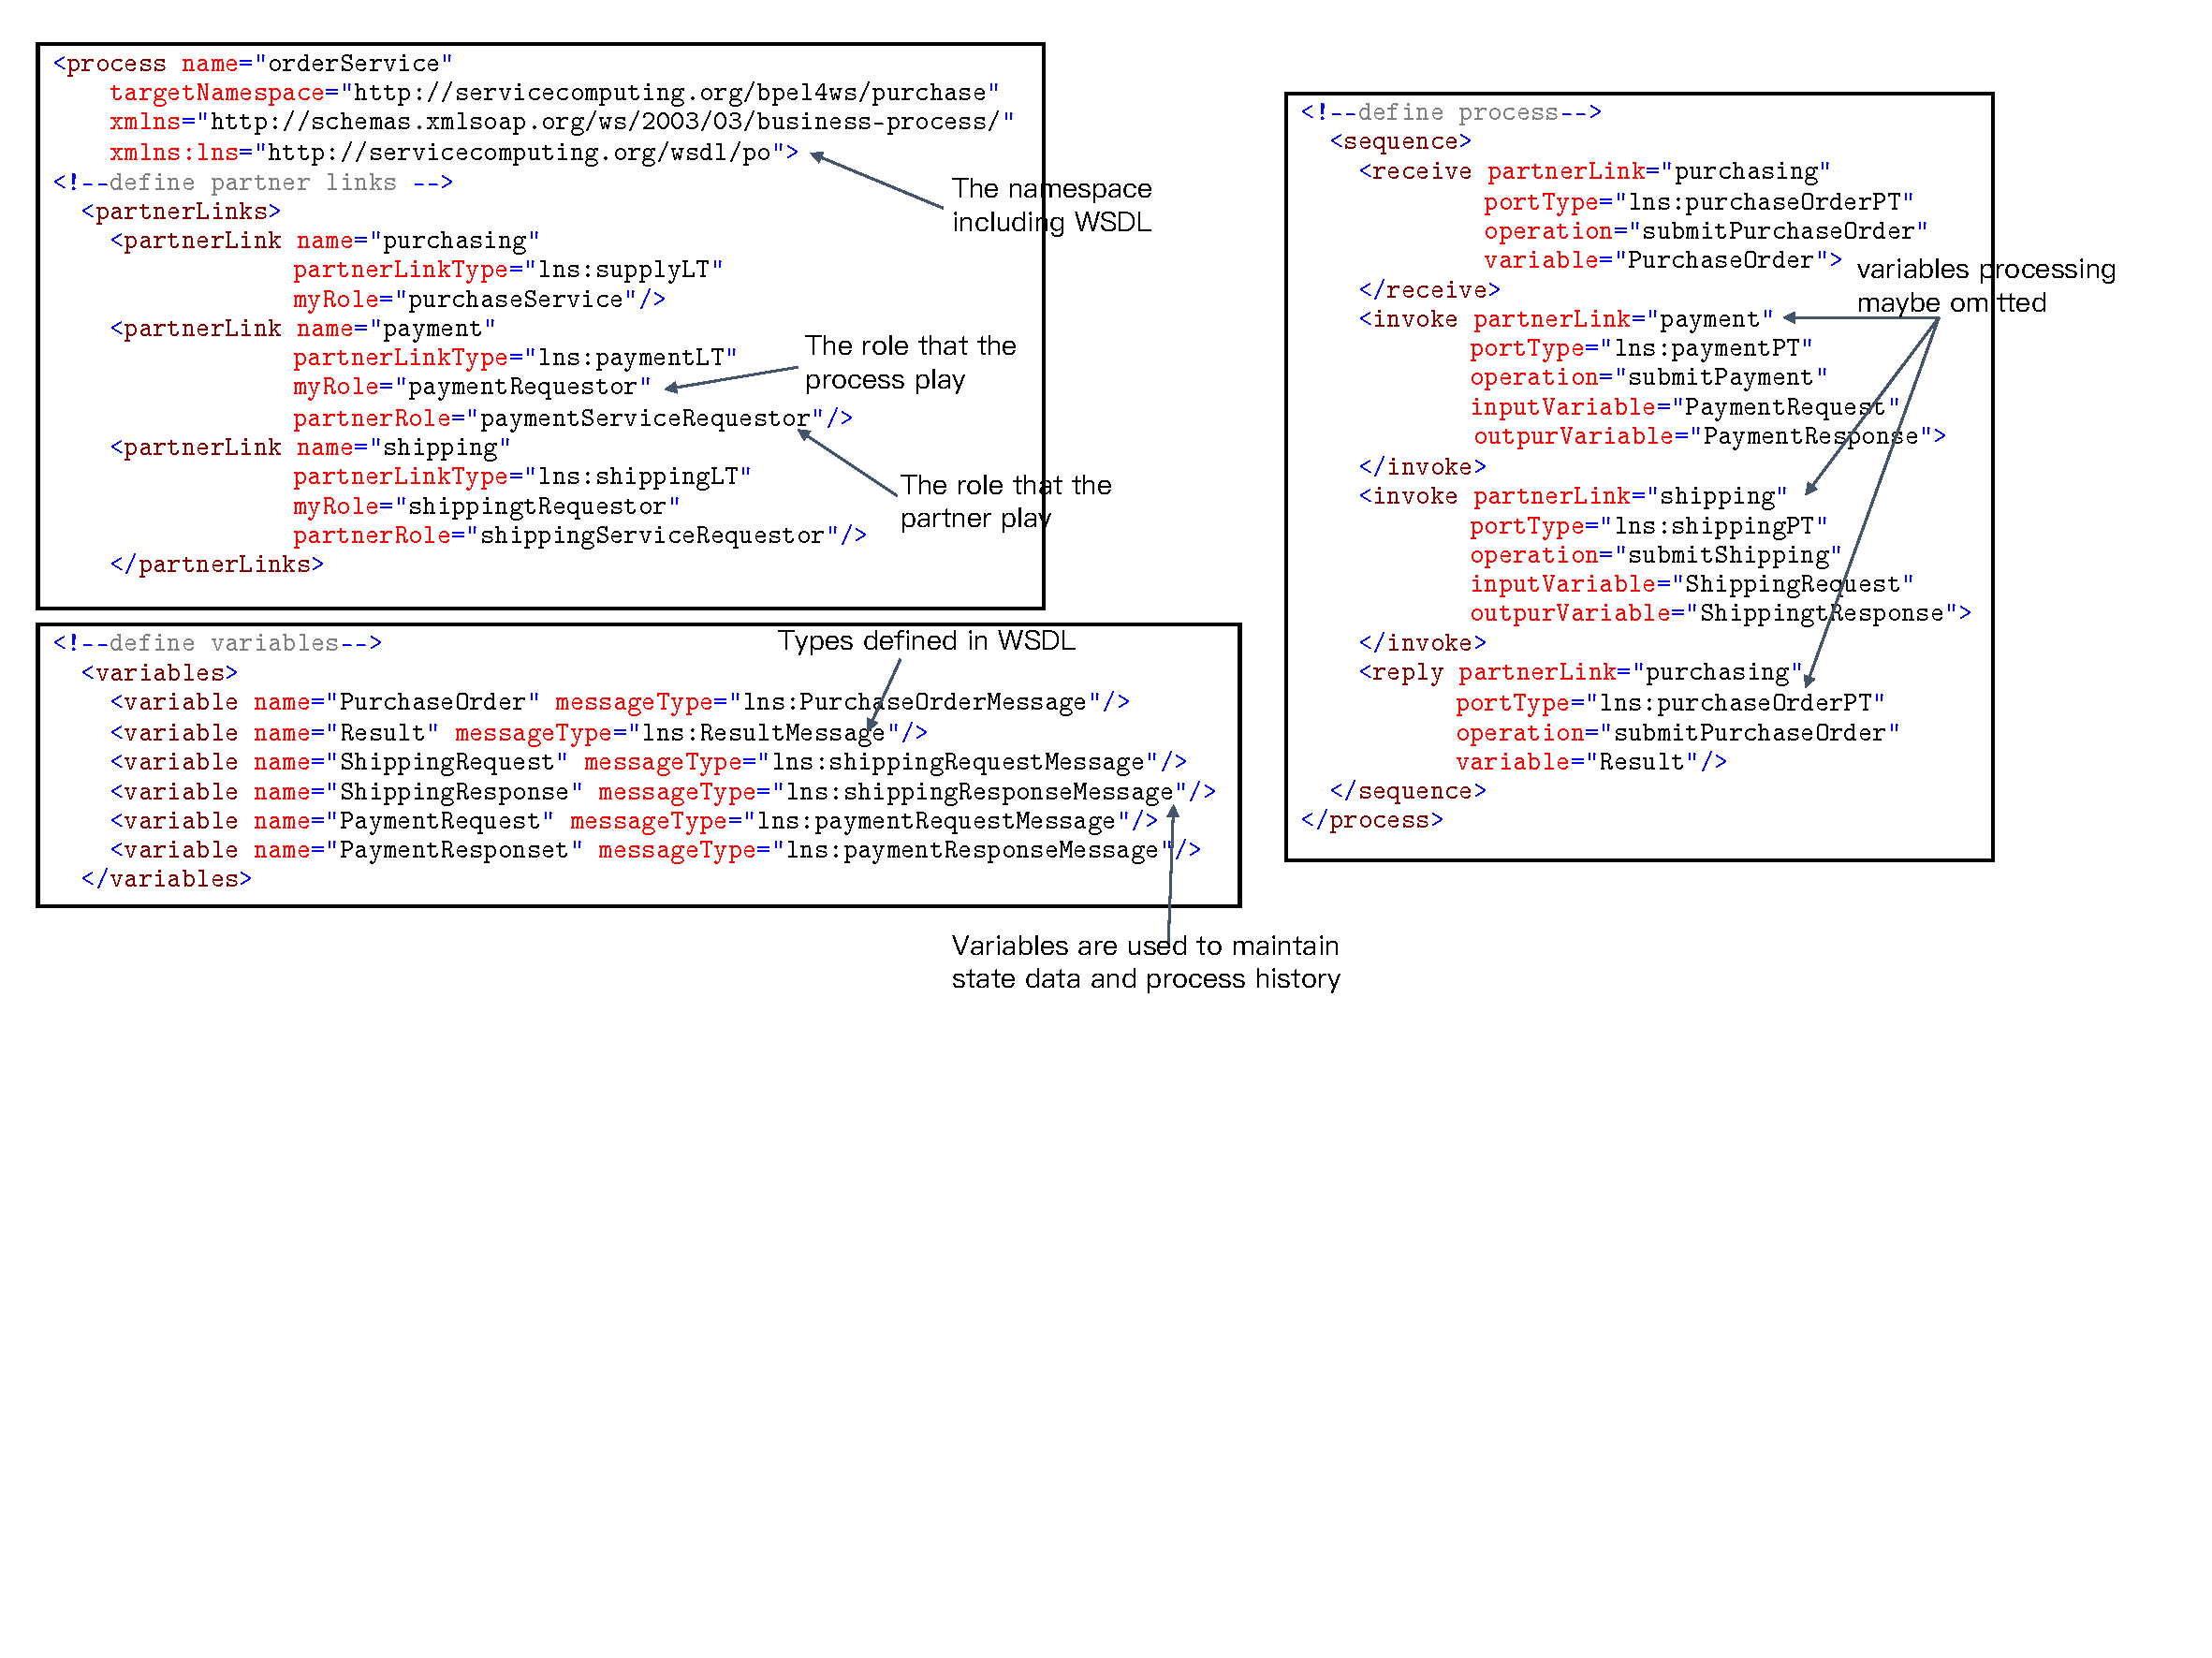
\includegraphics[width=\textwidth]{images/创建业务过程2.pdf}
    \vspace{-3em}
\end{figure}

\subsubsection{BPEL关键元素}

\vspace{-0.5em}
\begin{spacing}{1.2}
    \centering
    \begin{longtable}{|m{3.7cm}<{\centering}|m{11cm}|}
    \hline
    \textbf{element} & \multicolumn{1}{c|}{\textbf{描述}} \\ \hline
    partners &
    \vspace{-1.3em}
    \begin{itemize}[leftmargin=1.5em,itemsep=-2pt]
        \item 定义正在构建的业务流程与其合作流程之间的关系
        \item 合作伙伴可以作为
        \vspace{-0.2em}
        \begin{itemize}[leftmargin=1.5em,itemsep=-2pt]
            \item 提供业务流程所使用的服务的消费者
            \item 提供被业务流程使用的服务的提供者
            \item 激活业务流程的服务
        \end{itemize}
    \vspace{-1.5em}
    \end{itemize}                                           
    \\ \hline
    partner link types &
    \vspace{-1.3em}
    \begin{itemize}[leftmargin=1.5em,itemsep=-2pt]
        \item 定义两个Web服务之间的对话关系
        \item 在WSDL中定义,并给出与portType相关联的角色
    \vspace{-1.5em}
    \end{itemize}                                           
    \\ \hline
    partner links &
    \vspace{-1.3em}
    \begin{itemize}[leftmargin=1.5em,itemsep=-2pt]
        \item 对业务流程与其交互的合作伙伴服务进行建模
        \item 由partner link type所特征化
        \item 定义业务流程内的静态关系
    \vspace{-1.5em}
    \end{itemize}                                           
    \\ \hline
    business partners &
    \vspace{-1.3em}
    \begin{itemize}[leftmargin=1.5em,itemsep=-2pt]
        \item 使用partner元素对需要多个对话关系的业务合作伙伴关系进行建模
        \item 允许对partner links进行分组
        \item 禁止重叠
    \vspace{-1.5em}
    \end{itemize}                                           
    \\ \hline
    endpoint references &
    \vspace{-1.3em}
    \begin{itemize}[leftmargin=1.5em,itemsep=-2pt]
        \item 为服务提供端口特定数据提供动态绑定机制
        \item 允许将服务提供者与partner links中的角色进行动态绑定
    \vspace{-1.5em}
    \end{itemize}                                           
    \\ \hline
    activities &
    \vspace{-1.3em}
    \begin{itemize}[leftmargin=1.5em,itemsep=-2pt]
        \item 基本活动,例如接收、回复和调用
        \item 结构化活动
        \vspace{-0.2em}
        \begin{itemize}[leftmargin=1.5em,itemsep=-2pt]
            \item 按顺序执行(序列、开关和循环)
            \item 并发执行(流程)
            \item 非确定性选择(pick)
        \end{itemize}
        \item 属性,名称,连接条件,源,目标
    \vspace{-1.5em}
    \end{itemize}                                           
    \\ \hline
    data handling &
    \vspace{-1.3em}
    \begin{itemize}[leftmargin=1.5em,itemsep=-2pt]
        \item 在业务流程中建模状态
        \item 三种处理方式
        \vspace{-1em}
        \begin{multicols}{3}
        \begin{itemize}
            \item 变量
            \item 表达式
            \item 分配
        \end{itemize}
        \end{multicols}
        \vspace{-1.2em}
        \item 提供XML数据类型和WSDL消息类型
    \vspace{-1.5em}
    \end{itemize}                                           
    \\ \hline
    Correlation &
    \vspace{-1.3em}
    \begin{itemize}[leftmargin=1.5em,itemsep=-2pt]
        \item 用于处理进程之间长时间的有状态对话
        \item 用于识别新的业务流程
    \vspace{-1.5em}
    \end{itemize}                                           
    \\ \hline
    Scope &
    \vspace{-1.3em}
    \begin{itemize}[leftmargin=1.5em,itemsep=-2pt]
        \item 每个活动行为的上下文
        \item 共有五种:故障处理程序、事件处理程序、补偿处理程序、数据变量和相关性集
    \vspace{-1.5em}
    \end{itemize}                                           
    \\ \hline
\end{longtable}
\end{spacing}
\vspace{-1em}